
\part{Electromagnetismo}

\vspace*{\fill}

\begin{center}
	\textit{''El conocimiento es una red de ideas interconectadas, una vez que atrapamos una, las demás vienen detrás'' - Michael Faraday.}
\end{center}

\vspace*{\fill}

\chapter{Análisis Vectorial}
\dsnote{Solo se enunciarán los teoremas y propiedades más importantes.}
\section{Operadores Vectoriales}
\subsection{Gradiente}
El gradiente de un campo escalar es un campo vectorial. Es un vector normal a la curva de nivel en el punto estudiado
\begin{equation}
	\grad{f(r)} = \qty(\pdv{f}{x_1} \vu{x}_1 + \cdots + \pdv{f}{x_n} \vu{x}_n),
\end{equation}
Cuando $\grad{f} = 0$ se tiene un punto estacionario (máximo o mínimo). Dicho de otra forma, el gradiente marca la dirección en la cual varía más rápido el campo escalar y su magnitud indica cuan rápido varía. \\
\subsubsection{En Diferentes Sistemas de Coordenadas}
\begin{align*}
	\grad{\varphi} &= \pdv{\varphi}{r} \vu{r} + \frac{1}{r} \pdv{\varphi}{\theta} \vu{\theta} + \frac{1}{r\sin{\theta}} \pdv{\varphi}{\phi} \vu{\phi} \qquad \text{Coordenadas Esféricas} \\
	\grad{\varphi} &= \pdv{\varphi}{\rho} \vu{\rho} + \frac{1}{\rho} \pdv{\varphi}{\phi} \vu{\phi} + \pdv{\varphi}{z} \vu{z}.
\end{align*}
 


\subsection{Divergencia}
La divergencia de un campo vectorial mide la diferencia entre el flujo saliente y entrante en una región dada.
\begin{equation}
	\div{A} = \pdv{A_x}{x} + \pdv{A_y}{y} + \pdv{A_z}{z}.
\end{equation}
La divergencia produce un escalar, mide cuanto un vector se dispersa o sale de un punto.
\subsubsection{En Diferentes Sistemas de Coordenadas}
\begin{align*}
	\div{A} &= \frac{1}{r^2} \pdv{(r^2 A_r)}{r} + \frac{1}{r\sin{\theta}} \pdv{(\sin{\theta} A_\theta)}{\theta} + \frac{1}{r\sin{\theta}} \pdv{A_\phi}{\phi} \qquad \text{Coordenadas Esféricas} \\
	\div{A} &= \frac{1}{\rho} \pdv{(\rho A_\rho)}{\rho} + \frac{1}{\rho} \pdv{A_\phi}{\phi} + \pdv{A_z}{z} \qquad \text{Coordenadas Cilíndricas.}
\end{align*}








\subsection{Rotacional}
Operador vectorial sobre campos vectoriales: tendencia de un campo vectorial a inducir rotación.
\begin{equation}
	\curl{A} = \mqty| \vi & \vj & \vk \\ \pdv{x} & \pdv{y} & \pdv{z} \\ A_x & A_y & A_z |
\end{equation}


\section{Integración Vectorial}
Integrales de línea, superficie y volumen. Integrandos pueden ser vectores o escalares. \\
\subsection{Integrales de Línea}
Recorridos o trayectorias
\begin{equation}
	\int _c F(r) \cdot \dd{l}.
\end{equation}
Donde $F$ es un campo vectorial, $\dd{l}$ desplazamiento vectorial infinitesimal a lo largo de la curva y $c$ curva sobre la cual se integra. Cuando la integral de línea es independiente de la trayectoria el campo es conservativo.

\subsection{Integrales de Superficie}
Esta integral mide un flujo
\begin{equation}
	\int _S F\cdot \vu{n} \dd{a}
\end{equation}
Esto nos da un escalar. Si laintegral es cerrada $\oint F\cdot \vu{n} \dd{a}$.

\subsection{Teoremas Importantes}
\begin{teorema}
	\textbf{Teorema Fundamental de la Divergencia: }
	\begin{equation}
		\int _V \div{F} \dd{V} = \oint _S F\cdot \vu{n} \dd{a}.
	\end{equation}
\end{teorema}


\begin{teorema}
	\textbf{Teorema de Stokes: }
	\begin{equation}
		\int _S (\curl{F}) \cdot \vu{n} \dd{a} = \oint _c F \cdot \dd{l}.
	\end{equation}
\end{teorema}




\chapter{Electrostática}
Esta estudia los efectos mutuos que se producen entre los cuerpos como consecuencia de us carga eléctrica. La carga eléctrica es una propiedad fundamental y característica delas partículas elementales.
\begin{enumerate}
	\item La carga no se crea ni se destruye.
	\item Hay dos clases: positiva y negativa.
	\item En un sistema cerrado la carga se conserva.
\end{enumerate}

\section{Ley de Coulomb}
Experimentalemnte
\begin{enumerate}
	\item Dos cargas puntuales ejercen fuerza a lo largo de la línea que las une e inversamente proporcional al cuadrado de la distancia.
	\item La fuerza es proporcional al producto de las cargas.
\end{enumerate}

\begin{equation}
	\vec{F} = \frac{1}{4\pi \varepsilon _o} \frac{q_1 q_2}{r_{12} ^2} \vu{r}_{12}.
\end{equation}
Esto es válido para cargas puntuales, pero para muchas cargas se aplica el principio de superposición. Ahora, si la carga se distribuye en un volumen $V$ con densidad $\rho$ y sobre la superficie $S$ que limita $V$ con densidad $\sigma$, la fuerza ejercida por esta distribución de carga sobre una carga puntual $q$ está dada por:
\begin{align}
	F(r) &= \frac{q}{4\pi \ep} \int _V \rho (r') \frac{r - r'}{\abs{r - r'}^3} \dd{V'} + \frac{q}{4\pi \ep} \int _S \sigma (r') \frac{r - r'}{\abs{r - r'}^3} \dd{S'}.
\end{align}


\section{Campo Eléctrico}
Campo vectorial físico $\to$ región del espacio en la que interactúa la fuerza eléctrica. Se genera por cargas o campos magnéticos variables en el tiempo.
\begin{equation}
	\vec{E} (r) = \frac{1}{4\pi \ep} \sum _{i=1} ^N \frac{q_i}{r_i ^2} \vu{r} _i.
\end{equation}
Entonces, de manera general, tomando en cuenta distribuciones continuas de carga y cargas puntuales
\begin{equation}
	\vec{E} (r) = \kel \sum _{i=1} ^N q_i \frac{r - r_i}{\abs{r - r_i}^3} + \kel \int _V \frac{r - r'}{\abs{r - r'}^3} \rho (r') \dd{V'} + \kel \int _S \frac{r - r'}{\abs{r - r'}^3} \sigma (r') \dd{a'}
\end{equation}



\section{Potencial Electrostático}
El campo eléctrico cumple con
\begin{equation}
	\curl{\vec{E}} = 0.
\end{equation}
Sabemos que $\vec{E} (r) = -\grad{\varphi}$ es un potencial electrostático. Pero con esto se tiene
\begin{equation}
	\varphi (r) = -\int _{\mathcal{O}} ^r \vec{E} \cdot \dd{\vec{l}}
\end{equation}
donde $\mathcal{O}$ es el punto de referencia. Notemos que

\begin{enumerate}
	\item Potencial electrostático no es lo mismo que energía potencial.
	\item $\vec{E}$ es un vector derivado de un escalar y ya que $\curl{E} = 0$ esto implica: las componentes de $\vec{E}$ no son independientes
	\begin{equation}
		\pdv{E_x}{y} = \pdv{E_y}{x}, \qquad \pdv{E_z}{y} = \pdv{E_y}{z}, \qquad \pdv{E_x}{z} = \pdv{E_z}{x}.
	\end{equation}
	\item EL sistema de referencia es fundamental.
	\item El potencial obedece el principio de superposición.
	\begin{equation}
		\varphi (r) = \kel \sum_{i=1} ^N \frac{q_i}{\abs{r - r_i}} + \kel \int _V \frac{\rho (r')}{\abs{r-r'}} \dd{V'} + \kel \int _S \frac{\sigma (r')}{\abs{r - r'}} \dd{a'}.
	\end{equation}
\end{enumerate}

\section{Ley de Gauss}
Importante relación entre la integral de la componente normal del campo eléctrico sobre una superficie cerrada y la carga total encerrada por la superficie.
\begin{equation}
	\Psi _E = \int _S \vec{E} \cdot \vu{n} \dd{a}, \qquad \text{Flujo Eléctrica}
\end{equation}
Para una superficie cerrada imaginaria (superficie gaussiana). Se tiene que $\Psi _E \propto q$. Entonces
\begin{equation}
	\oint \vec{E} \cdot \vu{n} \dd{a} = \frac{1}{\ep} Q_{enc}.
\end{equation}
y por el teorema de la divergencia
\begin{equation}
	\div{\vec{E}} = \frac{\rho}{\ep}.
\end{equation}
A notar:
\begin{enumerate}
	\item Simetría esférica: Superficie gausiana $\to$ esfera concéntrica.
	\item Simetría cilíndrica: Superficie gaussiana $\to$ cilindro coaxial.
	\item Simetría palna: Superficie gaussiana $\to$ caja.
\end{enumerate}



\section{Dipolo Eléctrico}
Dos cargas iguales de signo contrario separados por una pequeña distancia. Supongamos una carga $-q$ en $r'$ y una carga $q$ en $r' + l$. Entonces
\begin{equation}
	\vec{E} (r) = \kel q \qty(\frac{r - r' - l}{\abs{r - r' - l}^3} - \frac{r - r'}{\abs{r - r'}^3})
\end{equation}
expandiendo el término de dentro
\begin{equation}
	\vec{E} (r) = \kel q \qty[\frac{3 (r - r') l}{\abs{r - r'}^3} (r - r') - \frac{l}{\abs{r - r'}} + \cdots]
\end{equation}

\subsection{Momento Dipolar Eléctrico}
Si se coloca un dipolo en un campo $\vec{E}$, ambas cargas $(q,-q)$ separadas una distancia $l$, experimentan fuerzas de igual magnitud y dirección contraria $\vec{F}$ y $-\vec{F}$, por ende: $\sum vec{F} = 0$ y $\sum \tau \neq 0$. Definimos el \textbf{momento dipolar} como $\vec{p} = q\vec{l}$. Por ende
\begin{align}
	\vec{E} (r) &= \kel \qty[\frac{3(r - r')\cdot \vec{p}}{\abs{r - r'}^3} (r - r') - \frac{\vec{p}}{\abs{r - r'}^3}].	\\
	\varphi (r) &= \kel q \qty[\frac{1}{\abs{r - r' - l}} - \frac{1}{\abs{r - r'}}] = \kel \frac{(r - r') \cdot \vec{p}}{\abs{r - r'}^3}.
\end{align}


\section{Trabajo y Energía en Electrostática}
Suponga una configuración de cargas estacionarias y se desea mover una carga de prueba $Q$ de un punto $a$ a un punto $b$. Por ende
\begin{equation}
	\varphi (b) - \varphi (a) = \frac{W}{Q}
\end{equation}
La diferencia de potencial entre $a$ y $b$ es igual al trabajo por unidad de carga requerido para mover $Q$ de $a\to b$.

\subsection{Energía de una Distribución de Cargas Puntuales}
Energía de la distribución $\to$ trabajo para ensamblar la distribución.
\begin{equation}
	W = \frac{1}{2} \sum_{i=1} ^n q_i \varphi (r_i).
\end{equation}
de otra forma se puede reescribir el trabajo
\begin{align}
	W &= \frac{\ep}{2} \qty[\oint _S \varphi \vec{E} \cdot \dd{a} + \int _V E^2 \dv{V}] \\
	W &= \frac{\ep}{2} \int _V E^2 \dv{V} \qquad \text{Si el volumen crece } (r\to \infty).
\end{align}





\chapter{Problemas Electrostáticos}

Estos problemas no son secillos de resolver. Por otro lado:
\begin{equation}
	\laplacian{\varphi} = -\frac{\rho}{\ep} \qquad \text{Ecuación de Poisson}.
\end{equation}

\textbf{Laplaciano:}
\begin{enumerate}
	\item \textbf{Rectangulares:}
	\begin{equation}
		\laplacian{\varphi} = \pdv[2]{\varphi}{x} + \pdv[2]{\varphi}{y} + \pdv[2]{\varphi}{z}.
	\end{equation}
	\item \textbf{Esféricas: }
	\begin{equation}
		\laplacian{\varphi} = \frac{1}{r^2} \pdv{r} \qty(r^2 \pdv{\varphi}{r}) + \frac{1}{r^2 \sin{\theta}} \pdv{\theta} \qty(\sin{\theta} \pdv{\varphi}{\theta}) + \frac{1}{r^2 \sin{\theta}} \pdv[2]{\varphi}{\phi}.
	\end{equation}
	\item \textbf{Cilíndricas: }
	\begin{equation}
		\laplacian{\varphi} = \frac{1}{\rho} \pdv{\rho} \qty(\rho \pdv{\varphi}{\rho}) + \frac{1}{\rho ^2} \pdv[2]{\varphi}{\theta} + \pdv[2]{\varphi}{z}.
	\end{equation}
\end{enumerate}

Y cuando interesa conocer el potencial en regones con $\rho = 0$.
\begin{equation}
	\laplacian{\varphi} = 0 \qquad \text{Ecuación de Laplace.}
\end{equation}

\section{Ecuación de Laplace}
\begin{teorema}
	Si $\varphi _1 ,\ldots ,\varphi _n$ son todas soluciones de la ecuación de Laplace, entonces:
	\begin{equation}
		\varphi = c_1 \varphi _1 + \cdots + c_n \varphi _n,
	\end{equation}
	con $c_i = $ ctes, también es solución de la ecuación de Laplace
	\begin{equation}
		\laplacian{\varphi} = c_1 \laplacian{\varphi}_1 + \cdots + c_n \laplacian{\varphi}_n = 0.
	\end{equation}
\end{teorema}


\begin{teorema}
	Dos sluciones de la ecuación de Laplace que satisfacen las mismas condiciones de frontera difieran a lo sumo en una constante aditiva.
\end{teorema}


\subsection{Ecuación de Laplace en una Dimensión}
Si $\varphi$ es una función de una variable. Las soluciones para cada uno de los sistemas importantes de coordenadas

\begin{enumerate}
	\item \textbf{Rectangulares:}
	\begin{equation}
		\varphi (x) = ax + b.
	\end{equation}
	\item \textbf{Esféricas: }
	\begin{equation}
		\varphi (r) = -\frac{a}{r} + b.
	\end{equation}
	\item \textbf{Cilíndricas: }
	\begin{equation}
		\varphi = a\ln{\abs{\rho}} + b.
	\end{equation}
\end{enumerate}

\subsubsection{Caso Esférico}
Para el caso esférico en dos dimensiones su solución luego de la separación de variables es
\begin{equation}
	\varphi (r,\theta) = \sum _{n=0} ^\infty \qty(A_n r^n + \frac{B_n}{e^{n+1}}) P_n (\cos{\theta}).
\end{equation}

\subsubsection{Caso Cilíndrico}
Ahora para el caso cilíndrico en dos dimensiones, su solución es:
\begin{equation}
	\varphi (\rho ,\theta) = A_o + B_o \ln{\abs{\rho}} + \sum _{n=1} ^\infty \qty(A_n \rho ^n + B_n \rho ^{-n}) \qty(C_n \cos{n \theta} + D_n \sin{n\theta}).
\end{equation}

\subsubsection{Caso Cartesiano}
Ahora la solución del caso cartesiano
\begin{equation}
	\varphi (x,y,z) = A e^{-(k + m) ^{1/2} x} \cos{m^{1/2} y} \cos{k^{1/2} z}.
\end{equation}

\section{Imágenes Electrostáticas}
Para un conujunto dado de condicioens de frontera, la solución a la ecuación de Laplace es única y resolviendo para $\varphi$ se ha encontrado la solución completa al problema. \\
El método de imágenes es un procedimiento para lograr este resultado sin resolver específicamente la ecuacioń diferencial. \dsnote{No se aplica universalmente, solo un número considerable de problemas (que bueno xd).} \\

Supongamos una carga $q$ arriba de un plano conductor: La carga $q$ inducirá una carga en el conductor. La potencia total a una distancia $\vec{r}$ estará dado por la contribución de la carga más la inducida en el conductor:
\begin{align*}
	\varphi (r) &= \varphi _1 (r) + \kel \int _S \frac{\sigma (r')}{\abs{r - r'}} \dd{a'}. \\
	\varphi (r) &= \varphi _1 (r) + \varphi _2 (r).
\end{align*}
$\varphi _2 (r)$ puede ser sustituído por un potencial debido a una distribución de carga especificada: 
\begin{itemize}
	\item Carga Imagen.
	\item Debe cumplir con las condiciones de frontera.
\end{itemize}


\subsection{Sistemas Conductores y Coeficientes de Potencial}
Cuando se tienen conductores con formas complicadas las soluciones analíticas quedan descartadas: Métodos numéricos. Se pueden sacar algunas conclusiones, supongamos $N$ conductores en una geometría fija:
\begin{itemize}
	\item Existe una relación lineal entre el potencial de un conductor y las cargas de los diversos conductores del sistema. $N$ conductores descargados excepto el conductor $j\to$ carga $Q_{jo}$. La solución de Laplace es el espacio fuera de los conductores la expresamos como:
	\begin{equation}
		\varphi _1 ^{(j)} (x,y,z) \quad \to \quad \text{potencial generado por } Q_{jo}.
	\end{equation}
	El potencial de cada uno de los conductores estará dado por:
	\begin{equation}
		\varphi _1 ^{(j)}, \ldots, \varphi _N ^{(j)}
	\end{equation}
	Reexpresando la carga del $j-$ésimo
	$$ \lambda Q_{jo}, \quad \lambda = \text{cte}, \quad \text{sadisface la ecuación de Laplace.} $$
	\item El potencial también se multiplica por $\lambda $.
	\item Todas las derivadas se multiplica por $\lambda$.
	\item $\sigma 0 -\ep \pdv{\varphi}{\vu{n}} \to$ todas las densidades se multiplican por $\lambda$.
	\item Potencial de cada conductor es proporcional a $Q_j$
	\begin{equation}
		\varphi _i ^j = p_{ij} Q_j, \qquad (i = 1,2,\ldots ,M)
	\end{equation}
	donde $p_{ij}$ es constante que depende de la geometría utilizando el mismo argumento para conductor $k$ $Q_k = \nu Q_{k_o}$ con $\nu =$ cte. Generalizando
	\begin{equation}
		\varphi _i = \sum _{j=1} ^{M} p_{ij} Q_j.
	\end{equation}
\end{itemize}









\chapter{Campo Electrostático en Medios Dieléctricos y su Teoría Microscópica}
Existen materiales conductoresy aislantes (dieléctricos)
\begin{itemize}
	\item Material dieléctrico ideal: material que no tiene cargas libres.
	\item Bajo la presencia de un campo eléctrico externo: pueden tener pequeños desplazamientos.
	\item Dieléctrico se polariza. Un dieléctrico polarizado es eléctricamente neutro, sin embargo produce un campo eléctrico en los puntos exteriores en interiores del dieléctrico. En un caso extermo, bajo un campo muy grande, ocurre la ionización. Un dipolo inducido $\vec{p} = \alpha \vec{E}$ donde $\alpha$ es la polarizabilidad atómica, depende de la estructura del átomo. Para moléculas es más complejo debido a que tienen direcciones preferenciales $\alpha \to \alpha _{ij}$.
\end{itemize}

\section{Polarización}
Consideremos un pequeño volumen $\Delta V$ de un medio dieléctrico que como todo es eléctricamente neutro. Si el medio está polarizado: Momento dipolar eléctrico
	\begin{equation}
		\Delta \vec{p} = \int _{\Delta V} r\dd{q}.
	\end{equation}
$\Delta \vec{p}$ depende del tamao del elemento de volumen. Se introduce el momento dipolar eléctrico por unidad de volumen y se conoce como polarización eléctrica:
\begin{equation}
	P \equiv \frac{\Delta \vec{p}}{\Delta V}.
\end{equation}
Momento dipolar de una molécula
\begin{equation}
	\vec{p} _m = \int _{\text{milecula}} r\dd{q}.
\end{equation}



\subsection{Campo Fuera de un Medio Dieléctrico}
Consideramos una porción finita de material dieléctrico polarizado. Esta polarización genera un campo eléctrico $\vec{E} \to \varphi$. Cada elemento de $\Delta V'$ se caracteriza por un momento dipolar $\Delta \vec{p} = P\Delta V'$ y tenemos $r \gg r'$. La contribución de las cargas en $\Delta V'$ al potencial está dada por:
\begin{equation}
	\Delta \varphi (r) = \kel \frac{\Delta p \cdot (r - r')}{\abs{r - r'}^3} = \kel \frac{P(r') \cdot (r - r') \Delta V'}{\abs{r - r'}^3}.
\end{equation}
El potencial total es la suma de todas las contribuciones de todas las partes del dieléctrico:
\begin{equation}
	\varphi (r) = \kel \int _{V_o} \frac{P(r') (r - r')}{\abs{r - r'}^3} \dd{V'}.
\end{equation}
Ahora buscamos encontrar $\vec{E}$
\begin{equation}
	\frac{r - r'}{\abs{r - r'}^3} = \nabla ^\prime \qty(\frac{1}{\abs{r - r'}}).
\end{equation}
Desarrollando la siguiente identidad: $\nabla ^\prime (f\vec{F}) = f\nabla ^\prime \cdot \vec{F} + \vec{F} \cdot \nabla ^\prime f.$ Se desarrolla la integral anterior, con ello se llega a 
\begin{equation}
	\varphi (r) = \kel \oint _{S_o} \frac{P \cdot \vu{n} \dd{a}}{\abs{r - r'}} + \kel \int _{V_o} \frac{(-\nabla ^\prime \cdot P) \dd{V}}{\abs{r - r'}}
\end{equation}
Con lo que se definen dos nuevas funciones escalares
\begin{itemize}
	\item $\sigma _p = P \cdot \vu{n}$.
	\item $\rho _p = -\div{P}$.
\end{itemize}

\begin{itemize}
	\item La densidad superficial de carga de polarización está dada por la componente de polarización normal a la superficie.
	\item La densidad de carga de polarización volumétrica es una medida de la no uniformidad de la polarización dentro del material.
\end{itemize}

Luego, calculando el campo eléctrico
\begin{equation}
	\vec{E} = \kel \qty[\int _S \sigma _p \frac{r - r'}{\abs{r - r'}^3} \dd{a'} + \int _{V_o} \rho _p \frac{r - r'}{\abs{r - r'}^3} \dd{V'}].
\end{equation}


\subsection{Campo Eléctrico dentro de un Dieléctrico}
En un dieléctrico la carga de prueba es comparable al tamaño de las moléculas. EL campo eléctrico dentro del dieléctrico debe tener las mismas propiedades. El campo eléctrico en un dieléctrico es igual al campo eléctrico dentro de una cavidad. \\

La ley de Gauss en un dieléctrico viene dada por
\begin{equation}
	\oint (\ep \vec{E} + \vec{P}) \cdot \vu{n} \dd{a} = Q.
\end{equation}
donde el término $\vec{D} = \ep \vec{E} + \vec{P}$ se le denomina \textbf{desplazamiento eléctrico}. 


\subsection{Suceptibilidad Dieléctrica y Constante Dieléctrica}
La polarización de un medio dieléctrico ocurre en respuesta al campo eléctrico en el medio. El grado de polarización depende:
\begin{itemize}
	\item Campo eléctrico
	\item Propiedades del material
\end{itemize}
A nivel macroscópico $F = P(E)$. En la mayoría de materiales $P$ se anula cuando $\vec{E} = 0$. Para materiales de este tipo y si son materiales siótropos, la polarización tendrá el mismo sentido que $\vec{E}$. 
\begin{equation}
	P = \chi (E) \vec{E} = \ep \chi _e \vec{E}.
\end{equation}
con esto se define $\varepsilon = \ep (1 - \chi _e)$.


\section{Condiciones de Frontera para los Vectores de Campo}
Variación de $\vec{E}$ y $\vec{D}$ al pasar por una zona interfacial entre dos medios. Considerando dos emdios encontacto y una densidad superficial de carga externa $\sigma$. Construir una pequeña superficie $S$: forma de caja de pastillas de altura despreciable. Entonces
\begin{equation}
	D_{2n} - D_{1n} = \sigma
\end{equation}
Observaciones
\begin{itemize}
	\item La discontinuidad en la componente normal $\vec{D}$ está dada por la densidad superficial de carga en la zona interfacial.
	\item Si no hay carga en la zona interfacial la componente normal de $\vec{D}$ no es contínua.
\end{itemize}
Y por la ley de Gauss se concluye que la componente tangencial del campo eléctrico es continua.
\dsnote{Después de toda esta parafernalia, el ejemplo clásico es el de la esfera dieléctrica en un campo eléctrico extermo, revisar el libro.}



\section{Teoría Microscópica de los Dieléctricos}
\subsection{Campo Molecular en un Dieléctrico: $E_m$}
Es el campo eléctrico en una posición molecular del dieléctrico el cual es producido por todas las fuentes externas y por todas las moléculas polarizadas del dieléctrico con excepción de la molécula en el punto considerado. El dieléctrico se polariza al inducir un campo. Suponemos polarización uniforma $\div{\vec{P}} = 0$. El campo eléctrico en el centro de la cavidad puede expresarse como:
\begin{equation}
	\vec{E}_m = \vec{E} _x + \vec{E}_d + \vec{E} _s + \vec{E} ^\prime
\end{equation}

\begin{itemize}
	\item $E_x$ campo eléctrico primario debido a los planos.
	\item $E_d$ campo debido a la carga de polarización e la superficie.
	\item $E_s$ campo debido a la carga de polarización en la superficie $S$.
	\item $E^\prime$ campo generado por dipolos dentro de $S$.
\end{itemize}


\subsection{Moléculas Polares}
\begin{itemize}
	\item Momento dipolar permanente
	\item Están formadas por al menos dos especcies distintas de átomos.
	\item En ausencia de campo eléctrico por una porción macroscópica del dieléctrico polar no está polarizada: dipolos individuales orientados al azar.
\end{itemize}
Si el dieléctrico polar se somete a un campo eléctrico, los dipolos se alinean con el campo. Si el campo es lo suficientemente intenso, la polarización alcanza el vapor de saturación: 
\begin{equation}
	P_s = N\vec{p}_m
\end{equation}
Se requiere valores de campo muy intensos. Si la temperatura se eleva la polarización disminuye. Según la mecánica estadística, a una temperatura $T$, la probabilidad de encontrar una molécula con energía $E$ es:
\begin{equation}
	f(E) = \propto e^{-E/kT}
\end{equation}
La energía potencial de un dipolo permanente $p_o$ en un campo eléctrico es:
\begin{equation}
	u = -p_o \cdot E_m
\end{equation}
La energía cinética de las moléculas no dependen del campo, entonces se desprecia su contribución en la distribución. El moemtno diplar efectivo de un dipolo molecular es su componente en la dirección del campo: $p_o \cos{\theta}$. El valor promedio de la cantidad está dado por:
\begin{equation}
	\expval{x}  =\sum x_m p_m = \frac{\sum _m \chi _m e^{-\beta e_m}}{\sum _m e^{-\beta u_m}}.
\end{equation}

pasando a lo continuo
\begin{equation}
	\expval{p_o \cos{\theta}} = p_o \qty(-\frac{1}{y} + \coth{y})
\end{equation}
con $y = p_o \frac{E_m}{kT}$ y a esta fórmula se le conoce como \textbf{Fórmula de Lagevin}. y el momento dipolar efectivo promedio
\begin{equation}
	\expval{p_o \cos{\theta}} = \frac{p_o ^2 E_m}{3kT}.
\end{equation}
Polarizabilidad por orientación $\alpha = \frac{p_o ^2}{3kT}$.

\begin{equation}
	\alpha = \alpha _o + \frac{p_o ^2}{3kT}
\end{equation}
a esta se le conoce como la \textbf{ecuación de Langevin-Debye}.

\subsection{Polarización Permanente: Ferroelectricidad}
Sabemos que
\begin{equation}
	E_m = E + \frac{p}{3\ep}
\end{equation}
Generalmente $E_m = 0$ cuando $E = 0$. Existen casos en los cuales $E = 0$ y $E_m = 0$ y esto se satisface para:
\begin{equation}
	p_o = 0, \qquad \frac{N \alpha}{3\ep} = 1.
\end{equation}
la cual es la condición de polarización permanente.






\chapter{Energía Electrostática}
Simplifica la resolución de algunos problemas. Y la contribución de energía de un sistema de cargas se divide en sus contribuciones cinética y potencial. \\
Energía potencial de un grupo de cargas puntuales
\begin{equation}
	u = \frac{1}{2} \sum _{j=1} ^{m} q_i \varphi _j.
\end{equation}
Energía electrostática de una distribució de carga:
\begin{align*}
	u &= \frac{1}{2} \ep \qty[\oint _S E\varphi \dd{a} + \int _V E^2 \dd{V}]. \\
	u &= \frac{1}{2} \int _V \rho (r) \varphi (r) \dd{V} + \frac{1}{2} \int _S \sigma (r) \varphi (r) \dd{a} + \frac{1}{2} \sum _j Q_j \varphi _j.
\end{align*}



\section{Condensadores}
Los condensadores son componentes eléctricos que sirven para almacenar energía. Dos conductores que puedan almacenar cargas iguales pero opuestas con una diferencia de potencial entre sí. La relación entre la carga almacenada y el potencial asociado es la capacitancia
\begin{equation}
	C \equiv \frac{Q}{\Delta \varphi}.
\end{equation}
Cuya energía se puede expresar como:
\begin{equation}
	u = \frac{1}{2} Q \Delta \varphi = \frac{1}{2} C \Delta \varphi ^2
\end{equation}
Si los conductores que forman un condensador tienen formas geométricas sencillas, la capacitancia puede obtenerse analíticamente. \\

Densidad de Energía:
\begin{equation}
	\mathcal{U} = \frac{1}{2} \ep E_o ^2 = \frac{1}{2} \ep \qty(\frac{Q}{\ep A})^2 = \frac{1}{2} \frac{Q^2}{\ep A^2}.
\end{equation}

Y para condensadores en circuitos paralelos y en serie\footnote{En paralelo se tiene la misma diferencia de potencial entre los nodos y para los circuitos en serie se conserva la carga.}

\begin{align*}
	C_{eq} &= C_1 + C_2, \qquad \text{Paralelo} \\
	\frac{1}{C_{eq}} &= \frac{1}{C_1} + \frac{1}{C_2}, \qquad \text{Serie.}
\end{align*}



\chapter{Corriente Eléctrica}
Carga en movimiento $\to$ corriente eléctrica. Proceso por el cual se transporta la carga $\to$ condicción. La corriente se define como la velocidad a la que se transporta la carga a través de una superficie dad e un sistema conductor
\begin{equation}
	I = \dv{Q}{t}.
\end{equation}
Por convención: el sentido en que se mueve los portadores positivos se toma como el sentido de la corriente. \\

Cosas a notar:
\begin{itemize}
	\item En gases la conducción es más complicada, ya que las poblaciones d eportadores varían mucho con condiciones experimentales.
	\item Al estar en equilibrio térico cada partícula tiene un movimiento aleatorio.
	\item Líquidos y gases $\to$ movimientos hidrodinámicos.
\end{itemize}

\section{Densidad de Corriente}
Consideremos un medio conductor con un solo tipo de portador de carga:
\begin{itemize}
	\item Sea $N$ un número de portadores de carga por unidad de volumen.
	\item Asumimos una velocidad $v$ para los portadores de carga.
\end{itemize}
Se define la densidad de carga como
\begin{equation}
	\vec{J} = \sum _i N_i q_i v_i.
\end{equation}
Cuya integral para una superficie da como resultado la corriente
\begin{equation}
	I = -\oint _S \vec{J} \cdot \vu{n} \dd{a} = -\int _V \div{\vec{J}} \dd{V} = \int _V \pdv{\rho}{t} \dd{V}.
\end{equation}
Lo que implica y da como resultado la \textbf{ecuación de la continuidad} y representa la \textbf{conservación de la carga}
\begin{equation}
	\pdv{\rho}{t} + \div{\vec{J}} = 0.
\end{equation}


\section{Ley de Ohm}
Para mantener una corriente se requiere de un campo eléctrico, por lo que la densidad de corriente es proporcional a la fuerza por unidad de carga
\begin{align}
    \vec{J} &\propto f \\
    \vec{J} = gf &= g\frac{\vec{F}}{q} \\
    \vec{J} &= g\vec{E}.
\end{align}
Donde $g$ es la conductividad. La ley de Ohm des esta forma es válida en medios lineales isótropos o medios óhmicos. Generalmente se usa el recíproco de $g$:
\begin{equation}
    \sigma = \frac{1}{g}.
\end{equation}
A lo cual se conoce como resistividad. Para un cable recto conductor y, utilizando la definición de corriente, se tiene
\begin{equation}
    \Delta \varphi = IR
\end{equation}
Y sabiendo que $P = \dv{W}{t}$, entonces
\begin{equation}
    P = I\Delta \varphi = I^2 R = \qty(\frac{\Delta \varphi ^2}{R}).
\end{equation}

\section{Corrientes Estacionarias en Medios Continuos}
Consideremos un medio conductor óhmico (lineal), homogéneo, en condiciones de conducción en estado estacionario, es decir con densidad de cargo local en equilibrio:
\begin{equation}
    \pdv{\rho}{t} (x,y,z) = 0
\end{equation}
Por ende la ecuación de continuidad se reduce a:
\begin{equation}
    \div{\vec{J}} = \div{g\vec{E}} = 0
\end{equation}
Para un medio homogéneo, $g$ no depende de $E$:
\begin{align*}
    g\div{\vec{E}} &= 0 \\
    \div{\vec{E}} &= -\laplacian{\varphi} = 0
\end{align*}
Por lo que el problema de conducción en estado estacionario puede resolverse. Se resuelve utilizando la siguientes condiciones de frontera:
\begin{itemize}
    \item Para estado estacionario: $\mqty{\div{\vec{J}} = 0 \\ J_{1n} = J_{2n}}$.
    \item La componente normal debe ser continua $g_1 E_{1n} = g_2 E_{2n}$, análogo a $D_N$.
    \item Puesto que el campo eléctrico es estático en cada medio $\mqty{\oint \vec{E} \cdot \dd{l} \\ E_{1t} = E_{2n}}$
\end{itemize}
Otra relación entre conducción y electrostática se da considerando dos electrodos metálicos en un medio infinito óhmico homogéneo de conductividad $g$. Los electrodos están a $\varphi _1$ y $\varphi _2$ respectivamente:
\begin{equation}
    I = \frac{\varphi _1 - \varphi_2}{R}
\end{equation}
reemplazando la definición de corriente en términos del campo eléctrico, se tiene
\begin{equation}
    RC = \frac{\varepsilon}{g}.
\end{equation}

\subsection{Aproximación al Equilibrio Electrostático}
Para un conductor el equilibrio se alcanza en poco tiempo. Entre menos conductor el equilibrio se alcanza más lento. Consideremos un medio isótropo, homogéneo, caracterizado por $g$ y $E$. Con densidad volumétrica de carga $\rho _o (x,y,z)$. Si se aísla repentinamente de los campos aplicados
\begin{equation}
    \pdv{\rho}{t} + \frac{g}{\varepsilon} \rho = 0
\end{equation}
Resolvemos la ecuación diferencial, por lo que se tiene
\begin{equation}
    \rho = \rho _o e^{-\frac{g}{\varepsilon} t}.
\end{equation}


\section{Redes de Resistencias y Leyes de Kirchhoff}
Los portadores de carga siguen una trayectoria de baja resistencia llamada circuito. 
\begin{itemize}
    \item Las fuerzas puramente electrostáticas no puede hacer circular una corriente en el circuito.
    \item Se necesita una diferencia de potencial externa $\Delta \varphi$.
\end{itemize}
Para resistencias en serie y paralelo, se conserva la corriente y el potencial respectivamente, y con ello se tiene
\begin{align}
    R &= R_1 + R_2 \qquad \text{Serie} \\
    \frac{1}{R} &= \frac{1}{R_1} + \frac{1}{R_2} \qquad \text{Paralelo}.
\end{align}
Cualquier sistema puede resolverse de forma sistemática por medio de las leyes de Kirchhoff:
\begin{enumerate}
    \item La suma algebraica de las diferencias de voltaje en cualquier malla\footnote{Trayectoria cerrada conductora en un circuito.} de la red es cero.
        \begin{equation}
            \sum \varphi _i = 0.
        \end{equation}
    \item La suma algebraica de las corrientes que circulan hacia un nodo\footnote{Pounto donde concurren tres o más conductores.} es cero.
        \begin{equation}
            \sum I_i = 0.
        \end{equation}
\end{enumerate}
Interpretando las leyes de Kirchhoff
\begin{enumerate}
    \item Reafirmación de
        \begin{equation}
            \oint \vec{E} \cdot \dd{l} = 0.
        \end{equation}
    \item Enunciado formal de conservación de la carga
        \begin{equation}
            \div{\vec{J}} = 0.
        \end{equation}
\end{enumerate}


\section{Teoría Microscópica de la Conducción}
Consideremos una partícula libre de carga $q$ y masa $m$, bajo la influencia de una fuerza eléctrica local, su velocidad de deriva aumentará:
\begin{equation}
    m\dv{v}{t} = q\vec{E}.
\end{equation}
Si la partícula se encontrara en el vacío continuará acelerándose. En un medio material donde pasa una corriente constante la velocidad sería constante. Debe existir una fuerza debido al medio
\begin{equation}
    m\dv{v}{t} = q\vec{E} - Gv
\end{equation}
Para una $v$ constante: $v_d = \frac{g\vec{E}}{G}$. Y para el caso general
\begin{equation}
    v(t) = \frac{g}{G} E \qty(1 - e^{-\frac{Gt}{m}}).
\end{equation}
Para el estado estacionario: $v_d = q\frac{E}{G} = q\frac{\tau}{m} E$. Si hay varios tipos de portadores de carga
\begin{equation}
    g = \frac{\sum N_i q_i ^2 \tau _i}{m_i}
\end{equation}
donde $\tau$ es aproximadamente entre colisiones del electrón de conducción; por ende, el reocorrido libre medio del electrón es:
\begin{equation}
    l = v_t \tau.
\end{equation}
con $v_t \gg v_d$. Para los materiales de mayor conductividad eléctrica, sólo se considera un tipo de portador de carga, el electrón:
\begin{align*}
    J &= N_e e v_d \\
    g &= N_e e^2 \frac{\tau}{m} = N_e e \frac{v_d}{E}
\end{align*}
con $\dfrac{v_d}{E}$ es la movilidad del electrón.




\chapter{El Campo Magnético de Corrientes Estacionarias}
Así como las cargas generan campos eléctricos, las corrientes generan campos magnéticos. Para esta sección haremos la densidad de carga y el campo eléctrico igual a cero, así solo nos concentramos en el campo magnético.

\section{Ley de Ampére}
La primera ecuación de la magnetostática es
\begin{equation}
    \curl{\vb{B}} = \mu _o \vb{J}
\end{equation}
esta es conocida como la \textbf{ley de Ampére}. Para el caso integral, tomamos una superficie abierta $S$ con borde $\partial S$. Se puede utilizar el teorema de Stockes para convertir la integral del rotacional a una integral de línea
\begin{equation}
    \int _S \curl{\vb{B}} \cdot \dd{\vb{S}} = \oint _{\partial S} \vb{B} \dot \dd{\vb{r}} = \muc \int _S \vb{J} \cdot \dd{\vb{S}}.
\end{equation}
por lo que
\begin{equation}
    \oint _{\partial S} \vb{B} \cdot \vb{r} = \muc I.
\end{equation}

\section{Vector Potencial}
Para distribuciones de corrientes simples se sabe que se tiene
\begin{equation}
    \div{\vb{B}} = 0.
\end{equation}
Pero para corrientes más generales esto no es el caso. Para garantizar una solución a la ecuación anterior se escribe el campo magnético en términos de algún campo vectorial.
\begin{equation}
    \vb{B} = \curl{\vb{A}}.
\end{equation}
Utilizando propiedades de los operadores vectoriales, la ley de Ampére se vuelve
\begin{equation}
    \curl{\vb{B}} = -\laplacian{\vb{A}} + \grad{(\div{\vb{A}})} = \muc \vb{J}
\end{equation}

\subsection{Mono-polos Magnéticos}
Pasamos muy rápido de la ley de Ampére a su representación en términos del potencial magnético, que no paramos a analizar la situación. Supongamos una especie de carga puntual $g$ sería fuente de campo magnético
\begin{equation}
    \vb{B} = \frac{g\vu{r}}{4\pi r^2}
\end{equation}
a esto se le conoce como \textit{mono-polo magnético}. Las ecuaciones de Maxwell dicen que esto no existe. Pero, qué tan tajante es esta conclusión? Estamos seguros qué no existen? En caso de que existan las ecuaciones de Maxwell no cambiarían significativamente, aunque la idea de $\vb{A}$ se perdería, pero, es esto algo tan importante? Pues en Mecánica Cuántica esto no es posible, existen propiedades que se pierden al perder $\vb{A}$ (buscar Aharonov-Bohm Effect). \\

Y aún así, es posible que existan mono-polos magnéticos y tener una ''versión'' del vector $\vb{A}$ que permita la presencia de esta carga magnética, pero solo si esta esta relacionada a la carga del electrón de la siguiente forma
\begin{equation}
    ge = 2\pi \hbar n, \quad n \, \in \, \Z.
\end{equation}
Esta es conocida como \textit{La Condición de Cuantización de Dirac.}

\subsection{Transformaciones de Gauge}
La elección de $\vb{A}$ no es única: existen muchos de potenciales vectoriales que dan como resultado el mismo campo magnético. Esto es debido a que el rotacional del gradiente es cero. Esto significa que se puede agregar cualquier vector potencial de la forma $\nabla _\chi$ para alguna función $\chi$ y el campo magnético se mantiene igual
\begin{equation}
    \vb{A}^\prime = \vb{A} + \nabla _\chi \quad \Rightarrow \quad \curl{\vb{A}^\prime} = \curl{\vb{A}}.
\end{equation}
Un cambio del vector $\vb{A}$ como este se denomina \textit{transformación de gauge}.

\begin{teorema}
    Siempre se puede encontrar una transformación de auge $\chi$ tal que $\vec{A} ^\prime$ que satisface $\div{\vb{A}^\prime} = 0$. A esto se le conoce como \textit{Coulomb gauge}.
\end{teorema}
Si necesitamos $\div{\vb{A}^\prime} = 0$, solo necesitamos que nuestra transformación gauge obedesca
\begin{equation}
    \laplacian{\chi} = -\psi .
\end{equation}
La cual siempre tiene solución dado que es una ecuación de Poisson. Existe otra cantidad a la que se le conoce \textit{potencial escalar magnético}, $\Omega$. La idea detras del potencial es que podemos estar interesados en conocer el campo magnético en una región donde no haya corrientes y el campo eléctrico no cambie en el tiempo. En este caso debemos resolver $\curl{\vb{B}} = 0$, lo que se puede hacer teniendo
\begin{equation}
    \vb{B} = -\grad{\Omega}.
\end{equation}
Esto es solo válido en un número limitado de situaciones, esto gracias a la no existencia de cargas magnéticas.


\subsection{Ley de Biot-Savart}
Ahora utilizaremos el vector potencial para resolver para el campo magnético en la presencia de una distribución de corriente. Por ahora siempre diremos que trabajaremos en Coulomb gauge y nuestro vector potencial obedece que $\div{\vb{A}} = 0$. Entonces la ley de Ampére se vuelve lo siguiente
\begin{equation}
    \laplacian{\vb{A}} = -\muc \vb{J}.
\end{equation}
Utilizamos la solución más general, las funciones de Green, se tiene
\begin{equation}
    \vb{A} (x) = \frac{\muc}{4\pi} \int _V \dd ^3 x^\prime \qty(\frac{\vb{J} (\vx ^\prime)}{\abs{\vx - \vx ^\prime}})
\end{equation}
necesitamos recordar que el índice

\subsubsection{El Campo Magnético}
Del resultado anterior se tiene $\vb{B} = \curl{\vb{A}}$. Aplicando y recordando que $\nabla$ actúa sobre $\vx$. Encontramos
\begin{equation}
    \vb{B} (\vx) = \frac{\muc}{4\pi} \int _V \dd ^3 \vx ^\prime \frac{\vb{J} (\vx ^\prime) \times (\vx - \vx ^\prime)}{\abs{\vx - \vx^\prime}^3}
\end{equation}
Esta es conocida como la \textbf{Ley de Biot-Savart}. Esto describe el campo magnético de una densidad de corriente general. 



\section{Dipolos Magnéticos}
\subsection{Corriente en una Espira}
Empezamos por un ejemplo clásico, una espira. Encontramos el campo magnético generado por una espira, utilizamos $\vb{r}$ en lugar de $\vx$. El vector potencial está como
\begin{equation}
    \vb{A} (\vb{r}) = \frac{\muc}{4\pi} \int _V \dd ^3 r^\prime \frac{\vb{J} (\vb{r^\prime})}{\abs{\vb{r} - \vb{r}^\prime}}
\end{equation}
Ahora, reemplazando por la corriente, se tiene
\begin{equation}
    \vb{A} (\vb{r}) = \frac{\muc I}{4\pi} \oint _C \frac{\dd{\vb{r}}^\prime}{\abs{\vb{r} - \vb{r} ^\prime}}
\end{equation}
Pensando como sería esto muy lejos de la espira, podemos expandir en Taylor el término de la integral y esto nos quedaría
\begin{equation}
    \vb{A} (\vb{r}) = \frac{\muc I}{4\pi} \oint _C \vb{r}^\prime \qty(\frac{1}{r} + \frac{\vb{r} \cdot \vb{r}^\prime}{r^3} + \cdots).
\end{equation}
\subsubsection{Momento Dipolar Magnético}
Teniendo el vector de superficie
\begin{equation}
    \mathcal{\mathbf{S}} = \int _S \dd{\vb{S}}
\end{equation}
y dado que el primer término de la ecuación del potencial magnético se anula por la inexistencia de mono-polos, se tiene
\begin{equation}
    \vb{A} (\vb{r}) = \frac{\muc}{4\pi} \frac{\vb{m} \times \vb{r}}{r^3}
\end{equation}
y con esto, introducimos el \textit{momento dipolar magnético} 
\begin{equation}
    \vb{m} = I\mathcal{\mathbf{S}}.
\end{equation}
Y con un poco de álgebra se tiene
\begin{equation}
    \vb{B} (\vb{r}) = \frac{\muc}{4\pi} \qty(\frac{3(\vb{m} \cdot \vu{r}) \vu{r} - \vb{m}}{r^3}).
\end{equation}


\section{Fuerzas Magnéticas}
Hasta ahora vimos que las corrientes producen campos magnéticos. Y sabemos que una partícula cargada con una velocidad $\vb{v}$ experimentará una fuerza
\begin{equation}
    \vb{F} = q\vb{v} \times \vb{B}.
\end{equation}
Esto significa que si una segunda corriente es situada en algún lugar de la vecindad de la primera, esta experimentará una fuerza de la otra.

\subsection{Fuerza entre Corrientes}
Para dos corrientes paralelas se tiene que la fuerza que siente una de ellas debido a la otra es
\begin{equation}
    \vb{F} = q\vb{v} \times \vb{B} = q\vb{v} \times \qty(\frac{\muc I_1}{2\pi d}) \mathbf{\otimes}.
\end{equation}

Y la fuerza por unidad de longitud es
\begin{equation}
    \vb{f} = -\qty(\frac{\muc I_1 I_2}{2\pi d}) \vu{x}.
\end{equation}

Y, de la ley de Biot-Savart se concluye que la forma general para la fuerza entre corrientes es
\begin{equation}
    \vec{F} = \frac{\muc}{4\pi} I_1 I_2 \oint _{C_1} \oint _{C_2} \dd{\vb{r}_2} \times \qty(\dd{\vb{r}_1} \times \frac{\vb{r}_2 - \vb{r}_1}{\abs{\vb{r}_2 - \vb{r}_1}^3}).
\end{equation}
En general, esta integral es ''tricky'' de resolver, pero si las corrientes están bien separadas es más sencillo expresar la fuerza en términos del momento dipolar magnético.


\subsection{Fuerza y Energía de un Dipolo}
Para encontrar esto se parte de
\begin{equation}
    \vb{F} = \int _V \dd ^3 r \vb{J} (\vb{r}) \times \vb{B} (\vb{r})
\end{equation}
\dsnote{luego de mucho cálculo se llega a }
\begin{align}
    \vb{F} &= \curl{(\vb{B} \times \vb{m})}, \\
    \vb{F} = \grad{\vb{B} \cdot \vb{m}}.
\end{align}
Y sabiendo que toda fuerza se puede expresar como el gradiente de una función, la función del dipolo en el campo magnético es
\begin{equation}
    U = -\vb{B} \cdots \vb{m}.
\end{equation}


\subsection{Fuerza entre Dipolos}
Tomando el caso en el que el campo magnético lo genera un dipolo $\vb{m} _1$. Sabemos que el campo magnético es de la forma
\begin{equation}
    \vb{B} (\vb{r}) = \frac{\muc}{4\pi} \qty(\frac{3(\vb{m}_1 \cdot \vu{r}) \vu{r} - \vb{m}_1}{r^3})
\end{equation}
Y, utilizando lo anteriormente encontrado, se tiene que la fuerza que siente el segundo dipolo es
\begin{equation}
    \vb{F} = \frac{\muc}{4\pi} \grad{\qty(\frac{3(\vb{m}_1 \cdot \vu{r}) (\vb{m}_2 \cdot \vu{r}) - \vb{m}_1 \cdot \vb{m}_2}{r^3})}
\end{equation}
donde $\vb{r}$ es el vector de $\vb{m}_1$ a $\vb{m}_2$. Y, notemos que la estructura de la fuerza es idéntica a la que hay entre dos dipolos eléctricos. Esto es particularmente satisfactorio dado que se utilizan dos métodos diferentes.



\chapter{Propiedades Magnéticas de la Materia}
\section{Magnetización}
A diferencia de la polarización eléctrica que es casi siempre en dirección de $\vb{E}$, algunos materiales adquieren su magnetización paralela a $\vb{B}$ (\textbf{paramagnéticos}) y algunos opuesta a $\vb{B}$ (\textbf{diamagnéticos}); solo unas pocas sustancias (como el hierro) retienen su magnetización incluso después de que el campo externo sea removido, a estos se le conocen como \textbf{ferromagnéticos.}

\subsection{Torques y Fuerzas en Dipolos Magnéticos}
Así como los dipolos eléctricos sienten un torque, y esto sucede de igual forma para el campo magnético
\begin{equation}
	\vb{N} = \vb{m} \times \vb{B}.
\end{equation}
\dsnote{En Griffiths no se ve del todo bien esto, revisar la parte de torque magnético en Zemansky, está mas de ahuevo la figura ahí.}
Y para un loop infinitesimal
\begin{equation}
	\vb{F} = \grad{\vb{m} \cdot \vb{B}}.
\end{equation}


\subsection{Magnetización}
En presencia de un campo magnético la materia se \textbf{magnetiza}, por el análisis microscópico, se sabe que se tienen muchos minidipolos que resultan alineados en cierta dirección.
\begin{equation}
	\vb{M} = \text{ momento dipolar magnético por unidad de volumen.}
\end{equation}
En otras palabras
\begin{equation}
	\vb{M} = \frac{\Delta \vb{m}}{\Delta V}.
\end{equation}



\section{El Campo de un Objeto Magnetizado}
\subsection{Límites de Corrientes}
Suponga que se tiene una pieza de material magnetizado; su momento dipolar magnético por unidad de volumen $\vb{M}$. El vector potencial es
\begin{equation}
	\vb{A} (\vb{r}) = \frac{\muc}{4\pi} \int \frac{\vb{M} (\vb{r} ^\prime) \times \vu{r}}{r^2} \dd{\tau ^\prime}
\end{equation}
con $\dd{\tau ^\prime}$ es un diferencial de volumen. Reemplazando $\frac{\vu{r}}{r^2} = \nabla ^\prime (\frac{1}{r})$, lo que resulta en
\begin{equation}
	\vb{A} (\vb{r}) = \frac{\muc}{4\pi} \int \frac{1}{r} \qty[\nabla ^\prime \times \vb{M} (\vb{r}^\prime)] \dd{\tau ^\prime} + \frac{\muc}{4\pi} \oint \frac{1}{r} \qty[\vb{M} (\vb{r}^\prime \times \dd{a^\prime})]
\end{equation}
El primer término es el potencial de una corriente volumétrica
\begin{equation}
	\vb{J} _b = \curl{\vb{M}}
\end{equation}
y el segundo es el potencial de una corriente superficial
\begin{equation}
	\vb{K} _b = \vb{M} \times \vu{n}.
\end{equation}
Esto es el análogo a la carga de volumen y superficie de polarización $\rho _b = -\div{\vb{P}}$ y $\sigma _b = \vb{P} \cdot \vu{n}$. Con todo esto, podemos expresar el campo magnético como
\begin{equation}
	\vb{B} (\vb{r}) = -\muc \grad{\varphi (\vb{r})} + \muc \vb{M} (\vb{r})
\end{equation}
donde $\varphi (\vb{r})$ es el campo escalar magnético \dsnote{Anteriormente lo introduje como $\Omega$, pero cambié de libro.} Y tiene la siguiente forma
\begin{equation}
	\varphi (\vb{r}) = \frac{1}{4\pi} \int _{V_o} \vb{M} (\vb{r} ^\prime) \cdot \frac{\vb{r} - \vb{r} ^\prime}{\abs{\vb{r} - \vb{r} ^\prime}^3} \dd{v} ^\prime.
\end{equation}

\subsection{Potencial Escalar Magnético y Densidad de Polos Magnéticos}
La expresión del potencial escalar magnético, es de forma parecida a la del potencial electrostático que provioene de un material dieléctrico polarizado. Utilizando la ecuación
\begin{equation}
	\frac{\vb{M} \cdot (\vb{r} - \vb{r}^\prime)}{\abs{\vb{r} - \vb{r} ^\prime}^3} = \vb{M} \cdot \nabla ^\prime \frac{1}{\abs{\vb{r} - \vb{r} ^\prime}} = \nabla ^\prime \cdot \frac{\vb{M}}{\abs{\vb{r} - \vb{r} ^\prime}} - \frac{1}{\abs{\vb{r} - \vb{r} ^\prime}} \nabla ^\prime \cdot \vb{M} .
\end{equation}
Y el potencial se reescribe como
\begin{equation}
	\varphi (\vb{r}) = \frac{1}{4\pi} \int _{S_o} \frac{\vb{M} \cdot \vu{n} \dd{a^\prime}}{\abs{\vb{r} - \vb{r}^\prime}} - \frac{1}{4\pi} \int _{V_o} \frac{\nabla ^\prime \cdot \vb{M}}{\abs{\vb{r} - \vb{r}^\prime}} \dd{v^\prime}.
\end{equation}
Con lo que se tiene
\begin{description}
	\item[Densidad de Polos Magnéticos: ] $\rho _M = -\nabla ^\prime \cdot \vb{M} (\vb{r} ^\prime)$.
	\item[Densidad Superficial de la Intensidad de Polos Magnéticos: ] $\sigma _M (\vb{r} ^\prime) = \vb{M} (\vb{r}^\prime) \cdot \vu{n}$.
\end{description}

\section{Fuentes de Campo Magnético: Intensidad Magnética}
Así como se tiene el desplazamiento eléctrico, definimos la \textbf{intensidad magnética} $\vb{H}$ como
\begin{equation}
	\vb{H} = \frac{1}{\muc} \vb{B} - \vb{M}.
\end{equation}
Combinando ecuaciones se tiene
\begin{equation}
	\vb{H} (\vb{r}) = \frac{1}{4\pi} \int _V \frac{\vb{J} \times (\vb{r} - \vb{r} ^\prime)}{\abs{\vb{r} - \vb{r} ^\prime}^3} \dd{v}^\prime - \grad{\varphi} (\vb{r}).
\end{equation}
Parece que no hemos ganado nada, dado que $\vb{H}$ aún depende de $\vb{M}$ a través de $\rho _m$ y $\sigma _m$. Más adelante se verá la relación entre esta nueva cantidad y la densidad de corriente. 


\section{Susceptibilidad y Permeabilidad Magnéticas e Histéresis}\footnote{En física, química y biología, la histéresis representa la tendencia de un material a conservar una de sus propiedades, en ausencia del estímulo que la ha generado.}
Para resolver problemas en la teoría magnética es esencial tener una relación entre $\vb{B}$ y $\vb{H}$. Estas relaciones depende de la naturaleza del material magnético y se obtienen generalmente a partir de experimentos. \\

En una extensa clase de materiales existe una relación aproximadamente lineal entre $\vb{M}$ y $\vb{H}$. Si el material es isótropo y también lineal.
\begin{equation}
    \vb{M} = \chi _m \vb{M}
\end{equation}
donde la cantidad escalar adimensional $\chi _m$ se llama \textit{susceptibilidad magnética}. Si $\chi _m$ es positiva, el material se llama \textit{paramagnético} y la inducción magnética se refuerza con la presencia del material. Si $\chi _m$ es negativa, el material es diamagnético y la inducción magnética se debilita con la presencia del material. Aunque $\chi _m$ es una función de la temperatura y a veces varía muy drásticamente con ella, generalmente puede decirse que, para materiales paramagnéticos y diamagnéticos, $\chi _m$ es bastante pequeña; es decir,
\begin{equation}
    \abs{\chi _m} \ll 1
\end{equation}
Una relación lineal entre $\vb{M}$ y $\vb{H}$ implica también una relación lineal entre $\vb{B}$ y $\vb{H}$:
\begin{equation}
    \vb{B} = \mu \vb{H}
\end{equation}
donde la permeabilidad $\mu$ se obtiene de la combinación de las ecuaciones
\begin{equation}
    \mu = \muc (1 + \chi _m)
\end{equation}
A veces se utiliza la \textit{permeabilidad relativa} en lugar de la permeabilidad $\frac{\mu}{\muc} = K_m$. Los materiales ferromagnéticos no son lineales, por lo que las ecuaciones anteriores no se aplican. \\


\section{Condiciones en la Frontera sobre los Vectores de Campo}
Ahora, como se hizo en electrostática, analizaremos como cambian los vectores $\vb{B}$ y $\vb{H}$ al pasar por una zona interfacial entre dos medios. Consideraremos dos medios en contacto, y realizando el análisis que se hizo en electrostática para medios dieléctricos, se tiene que la componente normal es continua
\begin{equation}
    \vb{B} _{2n} - \vb{B} _{1n} = 0.
\end{equation}
Y una condición de contorno del campo $\vb{H}$ puede obtenerse aplicando la ley de circuitos de Ampére. Con ello se obtiene
\begin{align}
    \qty(\vb{H}_2 - \vb{H}_1) &= \vb{j} \times \vu{n}_2 \\
    \vu{n} _2 \times \qty(\vb{H} _2 - \vb{H} _1) &= \vb{j}.
\end{align}




\chapter{Inducción Electromagnética}
\section{Inducción Electromagnética}
\begin{tcolorbox}
    Definiremos la \textit{fuerza electromotriz o fem}, alrededor de un circuito como
    \begin{equation}
        \oint _C \vb{E} \cdot \dd{\vb{l}} = \mathscr{E}.
    \end{equation}
\end{tcolorbox}
Con los campos $E$ y $B$ estáticos, esta fem siempre fue cero. Ahora veremos el caso donde no es nula. Como ahora $E$ no puede definirse a partir de la ley de Coulomb, es válido preguntarnos cómo se define. Se define de forma tal que la fuerza de Lorentz es siempre la fuerza electromagnética que actúa sobre una carga de prueba $q$.
\begin{equation}
    \vb{F} = q\qty(\vb{E} + \vb{v} \times \vb{B})
\end{equation}
Los resultados de un gran número de los experimentos realizados pueden resumirse asociando una fem inducida
\begin{equation}
    \mathscr{E} = -\dv{\Phi}{t}
\end{equation}
con un cambio en el flujo magnético que atraviesa por un circuito. Se encuentra que este resultado, conocido como \textbf{ley de Faraday de la Inducción Electromagnética}, es independiente de la forma en que cambia el flujo; el valor de $\vb{B}$ en distintos puntos interiores del circuito puede cambiar de muchas maneras. \\

Dadas las relaciones conocidas llegamos a la \textit{forma diferencial de la ley de Faraday}
\begin{equation}
    \curl{\vb{E}} = -\pdv{\vb{B}}{t}.
\end{equation}

\begin{tcolorbox}
    \textbf{\textit{Ley de Lenz}}. En caso de que haya un cambio en un sistema magnético, sucede algo que tiene a oponerse al cambio.
\end{tcolorbox}


\section{Autoinductancia}
El flujo magnético que atraviesa un circuito aislado depende de la forma geométrica del mismo y es linealmente dependiente de la intensidad de corriente en el circuito. Por tanto, para un circuito estacionario rígido, los únicos cambios de flujo resultan de cambios en la corriente
\begin{equation}
    \dv{\Phi}{t} = \dv{\Phi}{I} \dv{I}{t}.
\end{equation}
\begin{definition}
    La autoinductancai se define como:
    \begin{equation}
        L = \dv{\Phi}{I}.
    \end{equation}
    Y la ecuación con mayor importancia práctica es:
    \begin{equation}
        \mathscr{E} = -L\dv{\Phi}{t}.
    \end{equation}
\end{definition}



\section{Inductancia Mutua}
Solo se han considerado circuitos aislados, de modo que todo el flujo que se debía a la corriente en el propio circuito. Esta restricción puede eliminarse si se supone que hay $n$ circuitos. Entonces, en cualquier caso, lineal o no lineal, se tiene
\begin{equation}
    M_{ij} = \dv{\Phi_{ij}}{I_j}
\end{equation}
se define como la \textit{inductancia mutua} entre el circuito $i$ y el circuito $j$.


\section{La Fórmula de Neumann}
Para dos circuitos rígidos estacionarias en un medio lineal, la inductancia mutua es
\begin{equation}
    M_{21} = \frac{\Phi _{21}}{I_1}
\end{equation}
Esta ecuación es válida simplemente porque $\Phi _{21}$ es proporcional a $I_1$, lo que hace que $\Phi _{21} /I_1$ y $\dv{\Phi _{21}}{I_1}$ sean iguales. Ene este caso, se puede usar la ecuación para calcular $M_{21}$. El flujo está dado por
\begin{equation}
    \Phi _{21} = \frac{\muc}{4\pi} I_1 \int _{S_2} \left\{ \oint _{C_1} \frac{\dd{I_1} \times (\vb{r} _2 - \vb{r}_1)}{\abs{\vb{r} _2 - \vb{r}_1}^3} \right\} \cdot \dd{a}_2
\end{equation}
Sin embargo,
\begin{equation}
    \oint _{C_1} \frac{\dd{\vb{l}} \times (\vb{r}_2 \times \vb{r}_1)}{\abs{\vb{r}_2 - \vb{r}_1}^3} = \nabla _2 \times \oint _{C_1} \frac{\dd{\vb{l}}_1}{\abs{\vb{r}_2 - \vb{r}_1}}
\end{equation}
Con esto y el teorema de Stokes, se tiene
\begin{equation}
    M_{21} = \frac{\muc}{4\pi} \oint _{C_2} \oint _{C_1} \frac{\dd{\vb{l}}_1 \cdot \dd{\vb{l}}_2}{\abs{\vb{r}_2 - \vb{r}_1}}
\end{equation}
que se llama \textit{fórmula de Neumann} para la inductancia mutua. La simetría mencionada anteriormente es evidente de la ecuación. La fórmula de Neumann es igualmente aplicable a la autoinductancia, en cuyo caso se expresa como
\begin{equation}
    M_{21} = \frac{\muc}{4\pi} \oint _{C_2} \oint _{C_1} \frac{\dd{\vb{l}}_1 \cdot \dd{\vb{l}}_1 ^\prime}{\abs{\vb{r}_1 - \vb{r}_1 ^\prime}}.
\end{equation}

\section{Inductancias en Serie y Paralelo}
Podríamos proceder con una derivación basada simplemente en $\mathscr{E} = -L\dv{I}{t}$ y obtener fórmulas para la inductancia efectiva dejar de lado el hecho práctico de que un inductor siempre tiene cierta resistencia interna. Una inductancia perfecto es mucho más difícil de aproximar prácticamente que una capacidad perfecta o una resistencia perfecta. Por este motivo, las combinaciones en serie y paralelo, por ahora, contendrán siempre tanto resistencias como inductancias. Entonces, para una conexión en serie (se suman las caídas de potencial de cada elemento del circuito)
\begin{align}
    V &= R_1 I + L_1 \dv{I}{t} + M\dv{I}{t} + R_2 I + L_2 \dv{I}{t} + M\dv{I}{t} \\
    V &= \qty(R_1 + R_2) I + \qty(L_1 + L_2 + 2M) \dv{I}{t}.
\end{align}
El nuevo circuito contendrá una resistencia con magnitud $(R_1 + R_2)$ en serie con una inductancia $L_1 + L_2 + 2M$. Una expresión alternativa de la inductancia mutua es:
\begin{equation}
    M = k\sqrt{L_1 L_2}, \qquad -1\leq k \leq 1
\end{equation}
La inductancia efectiva esta dada por
\begin{equation}
    L_{ef} = L_1 + 2k\sqrt{L_1 L_2} + L_2.
\end{equation}
Para el caso de circuitos en paralelo en los que las resistencias son despreciables, el voltaje es el mismo y por ende, la inductancia efectiva
\begin{equation}
    L_{ef} = \frac{L_1 L_2 - M^2}{L_1 + L_2 - 2M} \dv{I}{t}.
\end{equation}




\chapter{Energía Magnética}
Establecer un campo magnético requiere un gasto de energía, lo cual se concluye directamente de la ley de inducción de Faraday. Si una fuente de voltaje $\mathscr{V}$ se aplica a un circuito, entonces la intensidad de corriente que pasa por el circuito puede expresarse con la ecuación
\begin{equation}
    \mathscr{V} + \mathscr{E} = IR
\end{equation}
donde $\mathscr{E}$ es la fem inducida y $R$ es la resistencia del circuito de corriente. Entonces se tiene
\begin{equation}
    \mathscr{V} \dd{q} = \mathscr{E} I\dd{t} + I^2 R \dd{t} = I\dd{\Phi} + I^2 R \dd{t}
\end{equation}
cuya última expresión se obtiene con la ayuda de la ley de Faraday. El último término representa la conversión irreversible de energía eléctrica en calor que se lleva a cabo el circuito, pero este término incluye todo el trabajo realizado por $\mathscr{V}$ sólo en los casos en los que el cambio de flujo sea cero. El otro término es el trabajo efectuado contra la fem inducida en el circuito. Es la parte del trabajo realizado por $\mathscr{V}$ que se invierte en alterar la estructura del campo magnético, con ello reescribimos
\begin{equation}
    \dd{W}_b = I\dd{\Phi}
\end{equation}
donde el subíndice $b$ indica que éste es el trabajo realizado por fuentes de energía eléctrica externas. 


\section{Energía Magnética de Circuitos Acoplados}
Si hay $n$ circuitos, entonces, según la ecuación anterior, el trabajo eléctrico hecho en contra de la fem inducidas está dado por
\begin{equation}
    \dd{W}_b = \sum _{i=1} ^n I_i \dd{\Phi}_i.
\end{equation}
En particular nos interesa el caso en el que los $\dd{\Phi _i}$ se producen por cambios de corriente en los mismos $n$ circuitos.
\begin{equation}
    \dd{\Phi}_i = \sum _{j=1} ^n \dv{\Phi _{ij}}{I_j} \dd{I_j} = \sum _{j=1} ^n M_{ij} \dd{I_j}.
\end{equation}
En caso de que sean circuitos rígidos y estacionarios, entonces no hay trabajo mecánico asociado a los cambios de flujo y el trabajo será igual al cambio en la energía magnética.
\begin{equation}
    U = \frac{1}{2} \sum _{i=1} ^n I_i \Phi _i
\end{equation}
La cual es la \textit{energía magnética} de $n$ circuitos acoplados y rígidos en medios lineales.

\section{Densidad de Energía en el Campo Magnético}
Es de interés una formulación alternativa de la energía magnética en función de los vectores de campo $\vb{B}$ y $\vb{H}$, porque proporciona una imagen en la que la energía se almacena en el campo magnético mismo. Tomando lo ya aprendido, otra forma de definir la energía
\begin{equation}
    U = \frac{1}{2} \int _V \vb{J} \cdot \vb{A} \dv{V}
\end{equation}
La última expresión puede transformarse aún más utilizando la ecuación de campo $\curl{\vb{H}} = \vb{J}$ y la identidad de la divergencia de un producto cruz, se tiene
\begin{equation}
    U = \frac{1}{2} \int _V \vb{H} \cdot \curl{\vb{A}} \dd{V} - \frac{1}{2} \int _S \vb{A} \times \vb{H} \cdot \vu{n} \dd{a},
\end{equation}
donde $S$ es la superficie que limita $V$. Eliminamos la integral de superficie extendiendo el volumen para que incluya todo el espacio, obtenemos
\begin{equation}
    U = \frac{1}{2} \int _V \vb{H} \cdot \vb{B} \dd{V}
\end{equation}
lo que da, claramente, como resultado lo siguiente
\begin{equation}
    u = \frac{1}{2} \vb{H} \cdot \vb{B}
\end{equation}
a lo que se conoce como \textit{densidad de energía} en un campo magnético.




\chapter{Corrientes que Varían Lentamente}
\section{Comportamiento Transitorio y en Estado Estacionario}
Es conveniente analizar el comportamiento de los circuitos en dos fases, dependiendo de si es importante el comportamiento periódico o el no periódico. El comportamiento periódico se llama comportamiento \textit{en estado estacionario}, mientras que el no periódico se conoce como comportamiento \textit{transitorio}. Ambos aspectos se rigen por las mismas ecuaciones básicas integro-diferenciales; sin embargo, las técnicas elementales usadas para resolverlas son radicalmente distintas en los dos casos.

\section{Leyes de Krichhoff}
Volviendo a enunciar las conocidas leyes de Kirchhoff
\begin{itemize}
    \item \textit{Ley de Kirchhoff I.} La suma algebraica de las corrientes instantáneas que fluyen hacia un nodo es cero.
    \item \textit{Ley de Kirchhoff II.} La suma algebraica de los voltajes aplicados instantáneos en una malla cerrada es igual a la suma algebraica de los contravoltajes instantáneos en la malla.
\end{itemize}
Para el circuito RLC más simple, el voltaje a lo largo del tiempo
\begin{equation}
    \mathscr{V} = RI + L\dv{I}{t} + \frac{1}{C} \int _{t_o} ^t I\dd{t}.
\end{equation}


\section{Comportamiento Transitorio Elemental}
El único comportamiento transitorio que consideraremos aquí es el asociado a la aplicación repentina de un voltaje constante $\mathscr{V}$ a una red de resistores, condensadores e inductores, siendo el primer ejemplo el circuito $R-L$. Para este circuito la ecuación es
\begin{equation}
    \mathscr{V} = RI + L\dv{I}{t}
\end{equation}
después de haber cerrado el interruptor $S$. La solución para la corriente es
\begin{equation}
    I(t) = \frac{\mathscr{V}}{R} \qty[1 - Ke^{-\frac{tR}{L}}].
\end{equation}
Volviendo a la ecuación integro-diferencial, se deriva respecto al tiempo
\begin{equation}
    \dv{\mathscr{V}}{t} = R\dv{I}{t} + L\dv[2]{I}{t} + \frac{1}{C}
\end{equation}
tomando la derivada del voltaje igual a cero, se tiene la siguiente solución
\begin{equation}
    I = \{ Ae^{i\omega _n t} + Be^{-i\omega _n t} \} e^{-\frac{Rt}{2L}}
\end{equation}
donde
\begin{equation}
    \omega _n = \sqrt{\frac{1}{LC} - \frac{R^2}{4L^2}}
\end{equation}
por lo que
\begin{equation}
    I(t) = De^{-\frac{Rt}{2L}} \sin{\omega _n t}.
\end{equation}

\section{Comportamiento en Estado Estacionario de un Circuito en Serie Simple}
Teniendo un circuito con el siguiente voltaje
\begin{equation}
    \mathscr{V} (t) = \mathscr{V}_o \cos{\omega t}.
\end{equation}
Este voltaje es la parte real de $\mathscr{V}_o e^{i\omega t}$, se desarrollará un método para encontrar la corriente física. Aplicamos al circuito un voltaje $\mathscr{V}_1 + i\mathscr{V}_2$, con esto se tiene
\begin{equation}
    \dv{\mathscr{V}_1}{t} + i\dv{\mathscr{V}_2}{t} = \qty(L\dv[2]{I_1}{t} + R\dv{I_1}{t} + \frac{I_1}{C}) + i\qty(L\dv[2]{I_2}{t} + R\dv{I_2}{t} + \frac{I_2}{C}).
\end{equation}
Usamos $\mathscr{V}_o e^{i\omega t}$ y la intensidad de corriente es $I_o e^{i\omega t}$, por lo que al reemplazar se tiene
\begin{equation}
    i\omega \mathscr{V}_o e^{i\omega t} = \qty[-\omega ^2 + i\omega + \frac{1}{C}] I_o e^{i\omega t}
\end{equation}
En donde $Z = R + i\omega L + \frac{1}{i\omega C}$ es la conocida como \textit{impedancia}. En esta la parte real es la resistencia \dsnote{la de toda la vida} y la parte imaginaria (\textit{reactancia} $X$) se divide en \textit{reactancia inductiva} $X_L$ y \textit{reactancia capacitiva} $X_C$. El hecho de que la impedancia sea compleja significa que la corriente no está en fase con el voltaje aplicado.

\section{Conexión de Impedancias en Serie y en Paralelo}
Así como ya se sabe, en serie el voltaje se suma, por ende, la impedancia efectiva es la suma de las impedancias
\begin{equation}
    Z = Z_1 + Z_2 + Z_3 + \cdots
\end{equation}
Es importante observar que las sumas de las impedancias son como números complejos
\begin{align*}
    Z &= Z_1 + Z_2 = (R_1 + R_2) + i(X_1 + X_2) \\
    Z &= \abs{Z} e^{i\theta}, \qquad \abs{Z} = \qty[(R_1 + R_2)^2 + (X_1 + X_2)^2]^{1/2} \\
    \theta &= \arctan{\frac{X_1 + X_2}{R_1 + R_2}}.
\end{align*}
Para las impedancias en paralelo el voltaje es el mismo, por ende
\begin{equation}
    \frac{1}{Z} = \frac{1}{Z_1} + \frac{1}{Z_2} + \dots
\end{equation}


\section{Potencia y Factores de Potencia}
la potencia suministrada a un resistor puede determinarse multiplicando el voltaje a través de cada resistor por la corriente que pasa a través de él. Sin embargo, para el caso más general.

\begin{tcolorbox}
	Si $V(t)$ e $I(t)$ son el voltaje y la corriente complejos, como se muestra, entonces la \textit{potencia instantánea} es
	\begin{equation}
		P(t) = \Re{I(t)} \Re{V(t)}.
	\end{equation}
	La \textit{potencia media} es una cantidad más importante, obtenida al tomar el promedio durante un periodo completo o durante un tiempo muy largo. Si las fases se escogen de tal modo que $V_o$ sea real y, como de costumbre, $Z = Ze^{i\theta}$, entonces es inmediato ver que
	\begin{equation}
		\bar{P} = \overline{\Re{I(t)} \Re{V(t)}} = \frac{1}{2} \abs{I_o} \abs{V_o} \cos{\theta}.
	\end{equation}
\end{tcolorbox}
Un factor un medio de la ecuación anterior representa el hecho de qeu el valor medio de $\sin ^2 {\omega t}$ o $\cos ^2 {\omega t}$ es un medio. EL otro factor interesante es el coseno de $\theta$, que tiene en cuenta el hecho de que la corriente y el voltaje no están en fase. El coseno de $\theta$ se llama frecuentemente \textit{factor de potencia} de un circuito de corriente alterna (CA)
\begin{equation}
	\overline{\Re{I_o e^{\omega t}} \Re{V_o e^{\omega t}}} = \frac{1}{2} \Re{I_o ^* V_o}.
\end{equation}
donde $I_o ^*$ es el conjugado de $I_o$. Entonces
\begin{equation}
	\bar{P} = \frac{1}{2} \frac{\abs{V_o}^2}{\abs{Z}^2} \Re{Z}
\end{equation}
Los valores eficaces del voltaje y de la corriente se definen normalmente como
\begin{equation}
	V_{ef} = \frac{\sqrt{2}}{2} \abs{V_o}, \qquad I_{ef} = \frac{\sqrt{2}}{2} \abs{I_o}
\end{equation}
La virtud de estas definiciones es que un $V_{ef}$ dado qeu se aplica a una resistencia disipa la misma potencia queun voltaje de la misma magnitud.





\chapter{Ecuaciones de Maxwell}
Ahora estamos listos para introducir la piedra angular de la teoría electromagnética, la llamada \textit{corriente de desplazamiento.} Aun cuando su efecto observable a veces es despreciable, es lo que completa esencialmente la teoría, y tiene un papel crucial en otros temas.

\section{Generalización de la Ley de Ampére: Corriente de Desplazamiento}
\begin{tcolorbox}
    La ley de Ampére ''corregida'' la podemos escribir de la siguiente forma
    \begin{equation}
        \curl{\vb{H}} = \vb{J} + \pdv{\vb{D}}{t}
    \end{equation}
    y nos referimos a la derivada respecto al tiempo de $\vb{D}$ como \textit{corriente de desplazamiento}.
\end{tcolorbox}
La introducción de la corriente de desplazamiento hace posible las ondas electromagnéticas, como veremos a continuación, y es la esencia de la gran contribución de Maxwell a la teoría electromagnético.

\section{Ecuaciones de Maxwell y sus Bases Empíricas}
Las ecuaciones de Maxwell en forma diferencial
\begin{align}
    \curl{\vb{H}} &= \vb{J} + \pdv{\vb{D}}{t} \label{ampere} \\
    \curl{\vb{E}} &= - \pdv{\vb{B}}{t} \label{faraday} \\
    \div{\vb{D}} &= \rho \label{gaussE} \\
    \div{\vb{B}} &= 0. \label{gaussM}
\end{align}



\section{Energía Electromagnética}
Ya se mostró que
\begin{align}
    U_E &= \frac{1}{2} \int _V \vb{E} \cdot \vb{D} \dd{V} \\
    U_M &= \frac{1}{2} \int _V \vb{H} \cdot \vb{B} \dd{V}.
\end{align}
Si se hace el producto escalar de la ecuación \eqref{ampere} por $\vb{E}$ y la ecuación resultante se resta del producto escalar de la ecuación \eqref{faraday} por $\vb{H}$, la ecuación que se obtiene es
\begin{equation}
    \vb{H} \cdot \curl{\vb{E}} - \vb{E} \cdot \curl{\vb{H}} = -\vb{H} \cdot \pdv{\vb{B}}{t} - \vb{E} \cdot \pdv{\vb{D}}{t} - \vb{E} \cdot \vb{J}
\end{equation}
el laod izquierdo se convierte en una divergencia\footnote{Usando la identidad: $\div{F\times G} = G\cdot \curl{F} - F\cdot \curl{G}$.}, entonces
\begin{equation}
    \div{(\vb{E} \times \vb{H})} = -\vb{H} \cdot \pdv{\vb{B}}{t} - \vb{E} \cdot \pdv{\vb{D}}{t} - \vb{E} \cdot \vb{J}
\end{equation}
Si estamos en medios lineales y el desplazamiento eléctrico y la intensidad magnética se puede escribir como su constante por el campo respectivo, se tiene
\begin{equation}
    \div{\vb{E} \times \vb{H}} = -\pdv{t} \frac{1}{2} \qty(\vb{E} \cdot \vb{D} + \vb{B} \cdot \vb{H}) - \vb{J} \cdot \vb{E}.
\end{equation}
Realizando la integral, se tomarán las siguientes abreviaturas
\begin{align}
    \vb{S} &= \vb{E} \times \vb{H} \\
    u &= \frac{1}{2} \qty(\vb{E} \cdot \vb{D} + \vb{B} \cdot \vb{H})
\end{align}
donde $\vb{S}$ se llama \textit{vector de Poyting}, entonces la ecuación anterior se reescribe como
\begin{equation}
    \div{\vb{S}} + \pdv{u}{t} = -\vb{J} \cdot \vb{E}.
\end{equation}
El término izquierdo es el trabajo realizado por el campo local sobre las partículas cargadas por unidad de volumen. También, $u$, se interpretó como la densidad de energía de los campos eléctricos y magnéticos. Si el trabajo es cero y la divergencia no es cero, se tiene
\begin{equation}
    \div{\vb{S}} + \pdv{u}{t} = 0.
\end{equation}
Dado que tiene la misma forma que una ecuación de continuidad, el término de la divergencia se toma con una razón de flujo de energía por unidad de área. Generalmente, $\vb{S} = \vb{E} \times \vb{H}$ se trata como el flujo local de energía por unidad de área.

\section{La Ecuación de Onda}
Tanto para $\vb{H}$ como para $\vb{E}$ se toma el rotacional de la ley de Ampére y la de Faraday. Con ello se tiene\footnote{Utilizando la identidad: $\curl{\curl} = \grad{\div} - \laplacian$}
\begin{align}
    \laplacian{\vb{H}} - \varepsilon \mu \pdv[2]{\vb{H}}{t} - g\mu \pdv{\vb{H}}{t} &= 0 \\
    \laplacian{\vb{E}} - \varepsilon \mu \pdv[2]{\vb{E}}{t} - g\mu \pdv{\vb{E}}{t} &= 0
\end{align}
Las ecuaciones de onda deducidas antes rigen el campo electromagnético en un medio lineal homogéneo en el que la densidad de carga es cero, sea este medio conductor o no. Al resolver las ecuaciones de onda, debe tenerse especial cuidado en obtener soluciones a las ecuaciones de Maxwell.

\section{Ondas Monocromáticas}
Las ondas monocromáticas son ondas en las que todos los campos están caracterizados por una sola frecuencia. En este caso, podemos resolver la ecuación de onda del campo eléctrico para encontrarlo y utilizar las ecuaciones de Maxwell y las relaciones constitutivas para encontrar los otros campos. Se considera que la dependencia del campo con respecto al tiempo es $e^{-i\omega t}$, de modo que
\begin{equation}
    \vb{E} (\vb{r},t) = \vb{E} (\vb{r}) e^{-i\omega t}
\end{equation}
Supondremos que el medio es el espacio vacío, de modo que $g=0$. Entonces se tiene
\begin{equation}
    \dv{\vb{E} (z)}{z} + \frac{\omega}{c} \vb{E} = 0
\end{equation}
donde $\ep \muc = 1/c^2$. Se conoce la solución al armónico simple
\begin{equation}
    \vb{E} (\vb{r} ,t) = \vb{E}_o \cos{\omega (t \mp z/c)}.
\end{equation}

En un dieléctrico no magnético y no conductor tomamos $\varepsilon = K\ep$, entonces se tiene
\begin{equation}
    \kappa = \sqrt{K} \omega/c.
\end{equation}
Definiendo $n = \sqrt{K}$ como \textit{índice de refracción} del medio dieléctrico.

\section{Condiciones de Frontera}
\dsnote{Para ahorrarnos la demostración, se mostrará solo la tabla de interés.}
\begin{table}[H]
    \centering
    \begin{tabular}{c||cccc}
        $g$ & $E_t$ & $D_n$ & $H_t$ & $B_n$ \\
        \hline
        \hline
        $g_1 = g_2 = 0$ & $E_{1t} = E_{2t}$ & $D_{1n} = D_{2n}$ & $H_{1t} = H_{2t}$ & $B_{1n} = B_{2n}$ \\ 
        $g_2 = \infty$ & $E_{2t} = 0$ & $D_{2n} = 0$ & $H_{2t} = 0$ & $B_{2n} = 0$ \\
         & $E_{1t} = 0$ & $D_{1n} = \sigma$ & $H_{1t} = j_\perp$ & $B_{1n} = 0$ \\
        $g_1 ,g_2 \, \text{arb} \neq \infty$ & $E_{1t} = E_{2t}$ & $\qty(\varepsilon _1 + i\frac{g_1}{\omega}) E_{1n}$ & $H_{1t} = H_{2t}$ & $B_{1n} = B_{2n}$ \\
         & & $= \qty(\varepsilon _2 + i\frac{g_2}{\omega}) E_{2n}$ & & \\
    \end{tabular}
    \caption{Condiciones de frontera.}
    \label{tab:boundaryCond}
\end{table}

\section{Ecuación de Onda con Fuentes}
Por lo que ya conocemos del campo magnético y la ecuación de faraday, se tiene
\begin{equation}
    \curl{\qty[\vb{E} + \pdv{\vb{A}}{t}]} = 0
\end{equation}
por lo que el término de dentro puede expresarse como el gradiente de un escalar
\begin{equation}
    \vb{E} = -\grad{\varphi} - \pdv{\vb{A}}{t}.
\end{equation}
Utilizando el mismo método que se utilizó anteriormente para  $\vb{H}$ y $\vb{E}$ se usa para $\vb{A}$
\begin{equation}
    -\laplacian{\vb{A}} + \varepsilon \mu \pdv[2]{\vb{A}}{t} + \grad{\div{\vb{A}}} + \varepsilon \mu \grad{\pdv{\varphi}{r}} = \mu \vb{J}.
\end{equation}
Se impone la llamada \textit{condición de Lorentz}
\begin{equation}
    \div{\vb{A}} + \varepsilon \mu \pdv{\varphi}{t} = 0
\end{equation}
se tiene una simplificación considerable. Si se satisface esta condición, entonces
\begin{equation}
    \laplacian{\vb{A}} - \varepsilon \mu \pdv[2]{\vb{A}}{t} = -\mu \vb{J}
\end{equation}
Y, con esto se tiene
\begin{equation}
    \laplacian{\varphi} - \varepsilon \mu \pdv[2]{\varphi}{t} = -\frac{1}{\varphi} \rho .
\end{equation}

Encontramos la solución \dsnote{Vease Reitz, p.410}
\begin{equation}
    \varphi (\vb{r} ,t) = \kel \int _V \frac{\rho (\vb{r} ^\prime, t^\prime)}{\abs{\vb{r} - \vb{r}^\prime}} \dd{v^\prime}
\end{equation}
donde $t^\prime = t - \frac{\abs{\vb{r} - \vb{r}^\prime}}{c}$ se llama \textit{tiempo de retardo}; $\varphi$ se llama \textit{potencial escalar retardado}. Ahora para el vector potencial
\begin{equation}
    \vb{A} (\vb{r} ,t) = \frac{\muc}{4\pi} \int _V \frac{\vb{J} (\vb{r}^\prime) ,t^\prime}{\abs{\vb{r} - \vb{r}^\prime}} \dd{v}^\prime
\end{equation}
que es el \textit{potencial vector retardado}.






\chapter{Propagación de Ondas Monocromáticas}
El término \textit{propagación de ondas electromagnéticas} cubre un amplio espectro de fenómenos físicos tales como ondas, luz visible y rayos $X$. En el vacío, todas las ondas se propagan a la misma velocidad $c$, pero se distinguen entre sí por sus frecuencias.

\section{Ondas Planas Monocromáticas en Medios no Conductores}
Las soluciones más ''fáciles'' sonlas que se conocen como soluciones de onda plana. Una onda plana se define como una onda que, en un instante dado, presenta la misma fase en todos los puntos que están sobre cada plano perpendicular a alguna dirección específica. Si, por ejemplo, la dirección especificada esla dirección $z$, entonces $\vb{E}$ debe tener la misma fase en todos los puntos que tienen el mismo valor de $x$, esto es, en todos los puntos en un plano paralelo al plano $xy$. Supongamos que se tiene que construir una solución de onda plana con una direcciónd e propagación $\vb{u}$, donde $\vb{u}$ es un vector unitario. Entonces la variable $z$ en el exponente debe cambiarse por $\vb{u} \cdot \vb{r}$, la proyección de $\vb{r}$ en la dirección de $\vb{u}$. Por tanto, una onda plana con dirección de propagación $\vb{u}$ se representa como
\begin{align*}
	e^{-i(\omega t - \kappa \vb{u} \cdot \vb{r})}
\end{align*}
Definiremos un \textit{vector de propagación}
\begin{align*}
	\vb{\kappa} &= \kappa \vb{u}.
\end{align*}
La velocidad de propagación de una onda plana monocromática es precisamente la velocidad con la que se mueven los planos de fase constante. Obviamente, por fase constante queremos decir que
\begin{equation}
	\vb{\kappa} \cdot \vb{r} - \omega t = \text{ cte}
\end{equation}
Si $\vb{\kappa} \cdot \vb{r}$ se escribe como $\kappa \xi$, siendo $\kappa$ la magnitud de $\vb{\kappa}$ y $\xi$ como la proyección de $\vb{r}$ en la dirección $\vb{\kappa}$, entonces la ecuación anterior se convierte en 
\begin{equation}
	\kappa \xi - \omega t = \text{ cte}.
\end{equation}
Derivando con respecto al tiempo y utilizando $\kappa = \frac{n\omega}{c}$, encontramos la velocidad de fase
\begin{equation}
	v_p = \frac{c}{n}
\end{equation}
en el espacio libre $v_p = c$. \\


Ahora tomando las ecuaciones de Maxwell para donde no hay distribuciones de carga ni de corrientes y la conductividad es $g=0$. Se tiene que $\pdv{t} = i\omega$ y $\nabla = i\vb{\kappa}$, por lo que, las ecuaciones de Maxwell para ondas planas se transforman en
\begin{align}
	\vb{\kappa} \cdot \vb{D} &= 0 \\
	\vb{\kappa} \cdot \vb{B} &= 0 \\
	\vb{\kappa} \times \vb{E} &= \omega \vb{B} \\
	\vb{\kappa} \times \vb{H} &= -\omega \vb{D}.
\end{align}

\begin{tcolorbox}
	Recordando las ecuaciones consitutivas para medios lineales
	\begin{align}
		\vb{D} &= \varepsilon \vb{E} \\
		\vb{H} &= \frac{1}{\mu} \vb{B}.
	\end{align}
\end{tcolorbox}
Consideramos tambíen que el medio es homogéneo e isótropo, de modo que $\varepsilon$ y $\mu$ son escalares constantes. Y todo será en medios no magnéticos
\begin{align}
	K\vb{\kappa} \cdot \vb{E} &= 0 \\
	\vb{\kappa} \cdot \vb{B} &= 0 \\
	\vb{\kappa} \times \vb{E} &= \omega \vb{B} \label{faraday2} \\
	\vb{\kappa} \times \vb{B} &= -\frac{\omega}{c^2} K\vb{E}. \label{ampere2}
\end{align}
Priemro, si suponemos $K\neq 0$, vemos que $\vb{\kappa} \cdot \vb{E} = 0$ ; $\vb{\kappa}\ cdot \vb{B} = 0$ siempre. Ambos campos deben ser perpendiculares a $\vb{\kappa}$. Tal onda se llama \textit{onda transversal.} Aplicando el vector $\vb{\kappa}$ a \eqref{faraday2} y reemplazando \eqref{ampere2} y tomando la condición de ondas transversales
\begin{equation}
	K\frac{\omega ^2}{c^2} \vb{E} = \kappa ^2 \vb{E}.
\end{equation}
lo que es equivalente a la ecuación de onda para soluciones de la forma dada por la \eqref{ampere2}, con lo que se tiene
\begin{equation}
	\kappa = \sqrt{K} \frac{\omega}{c}
\end{equation}
esta relaciń, llamada \textit{relación de dispersión transversal}, determina la magnitud el vector de onda $\vb{\kappa}$ en términos de las $\omega$ y $K$ supuestas.


\begin{tcolorbox}
	Onda monocromática transversal que se propaga en dirección positiva de $\vb{u}$ está descrita por
	\begin{equation}
		\vb{E} (\vb{r},t) = \vu{E} e^{-i(\omega t -\vb{\kappa} \cdot \vb{r})}, \qquad \vb{B} (\vb{r},t) = \vu{B} e^{-i(\omega t - \vb{\kappa} \cdot \vb{r})}.
	\end{equation}
	La dirección $\vb{u}$ y la frecuencia $\omega$ son completamente arbitrarias. La amplitud $\vb{E}$ es arbitraria, excepto que debe ser perpendicular a $\vb{u}$: $\vb{u} \cdot \vb{E}$. Entonces $\vu{B}$ está completamente determinado en magnitud y dirección: 
	\begin{equation}
		\vu{B} = \frac{n}{c} \vb{u} \times \vu{E}.
	\end{equation}
	Para varias ondas, se tiene la superposición de ondas
	\begin{equation}
		\vb{E} (\vb{r},t) = \sum _i \vu{E} (\vb{\kappa} _i,\omega _i) \exp{-i(\omega _i t - \vb{\kappa}_i \cdot \vb{r})}
	\end{equation}
	Para una solucion que no sea periódica, la suma puede convertirse en una integral en donde la función $\vu{E} (\vb{\kappa},\omega)$ se llama \textit{transformada de Fourier}.
\end{tcolorbox}







\section{Polarización}
Es una propiedad de las ondas que puede oscilar con más de una orientación. Esto se refiere normalmente a las llamadas ondas transversales. \\
Descomponiendo el vector $\vb{E}$ como suma de un vector paralelo al plano de incidencia y un vector perpendicular a dicho plano
\begin{equation}
	\vb{E} = E_\parallel e^{i\theta_\parallel} \vu{u} _\parallel + E_\perp e^{i\theta_\perp} \vu{u}_\perp.
\end{equation}
Se realiza la diferencia $\theta _\parallel - \theta _\perp$ y según el resultado se tendrá:
\begin{description}
	\item[Polarización lineal: ] Si la diferencia es $0$ o un múltiplo entero de $\pi$.
	\item[Polarización circular: ] Si la diferencia es un múltiplo entero impar de $\frac{\pi}{2}$. En este caso se cumple, además, que $E_\parallel = E_\perp$.
	\item[Polarización elíptica: ] Para el resto de casos. Es posible conocer el sentido de giro de la polarización de la onda a partir de la diferencia anterior 
	\begin{itemize}
		\item Si $\theta _\parallel - \theta _\perp < 0$ se trata de \textit{polarización elíptica lovógira} o helicidad negativa (en contra de las agujas del reloj).
		\item Si $\theta _\parallel - \theta _\perp > 0$ se trata de \textit{polarización elíptica dextrógira} o helicidad positiva (a favor de la agujas del reloj).
	\end{itemize}
\end{description}



\chapter{Formularios}
Formularios proporcionados por los catedráticos: Dr. Rodrigo Sacahuí y Lic. Héctor Pérez
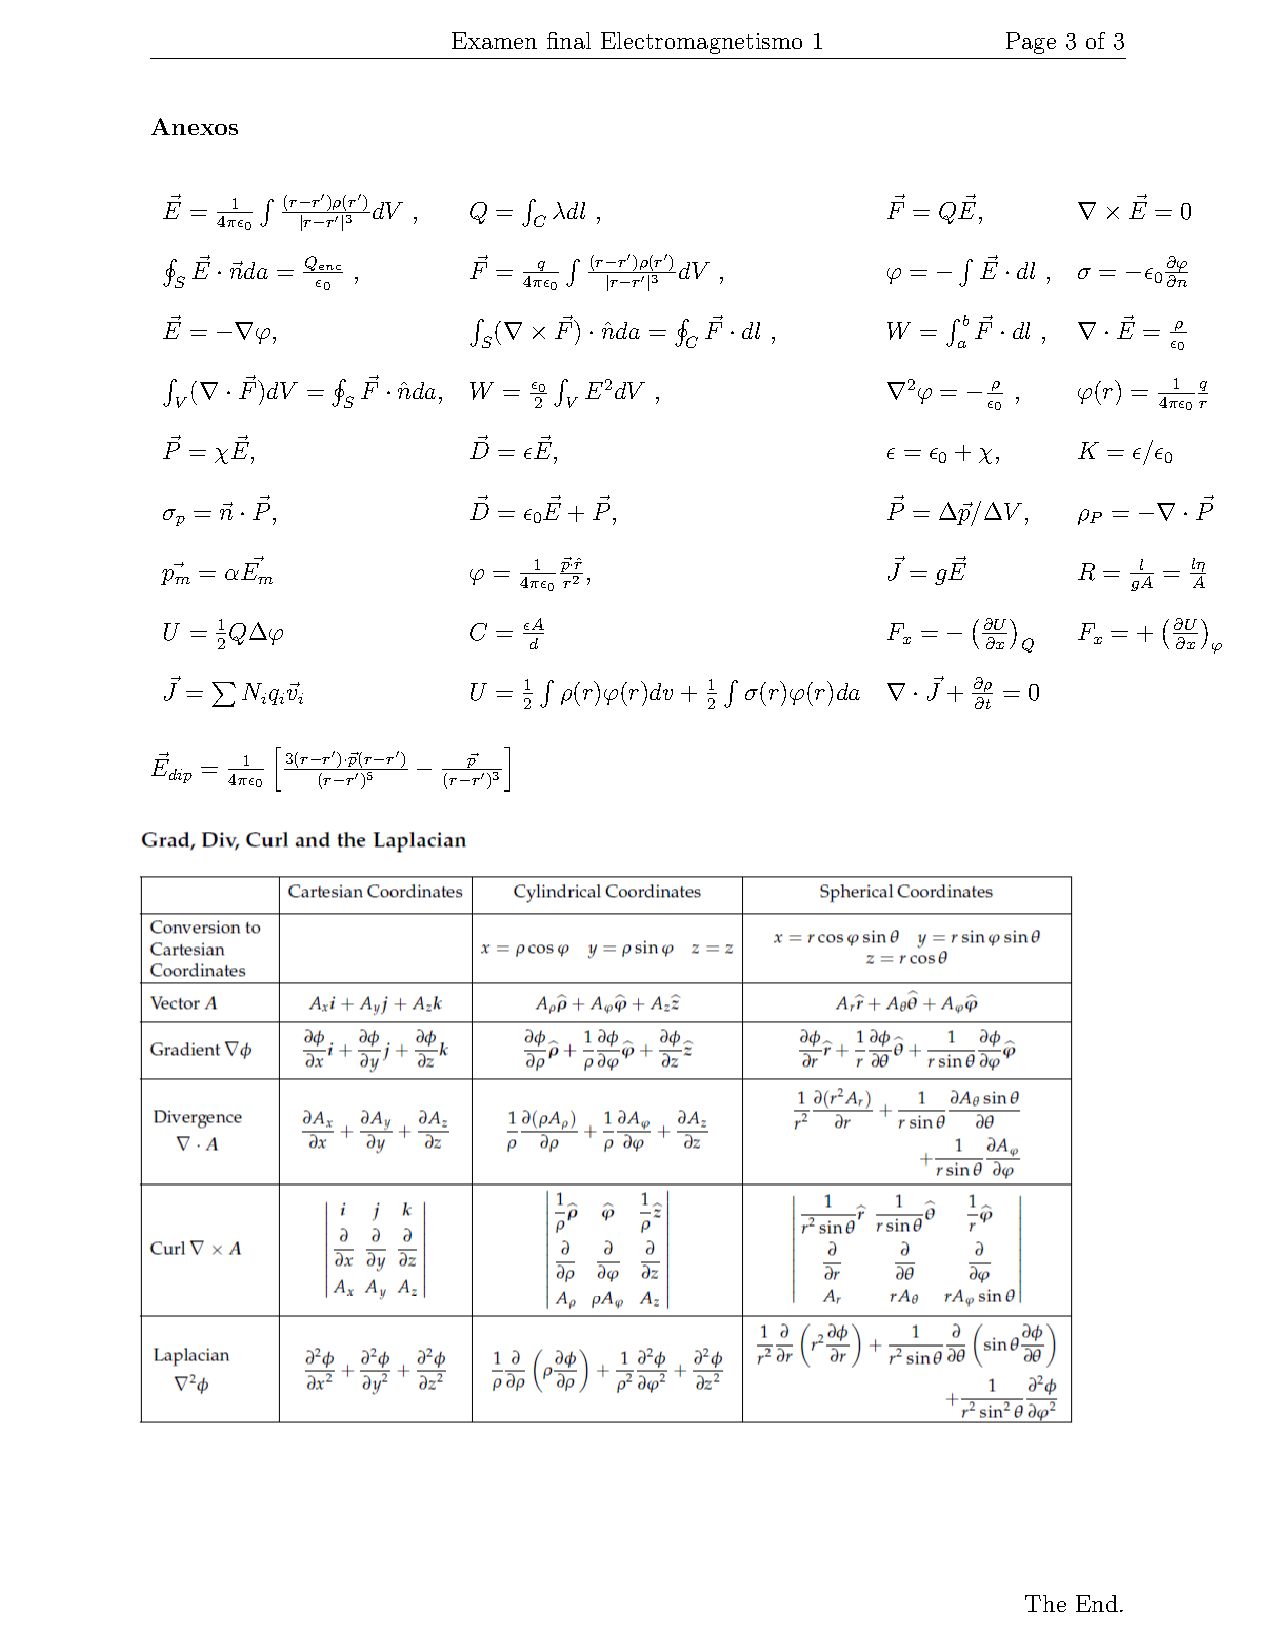
\includepdf[pages=-, scale=0.9]{./img/formulario_electro1.pdf}
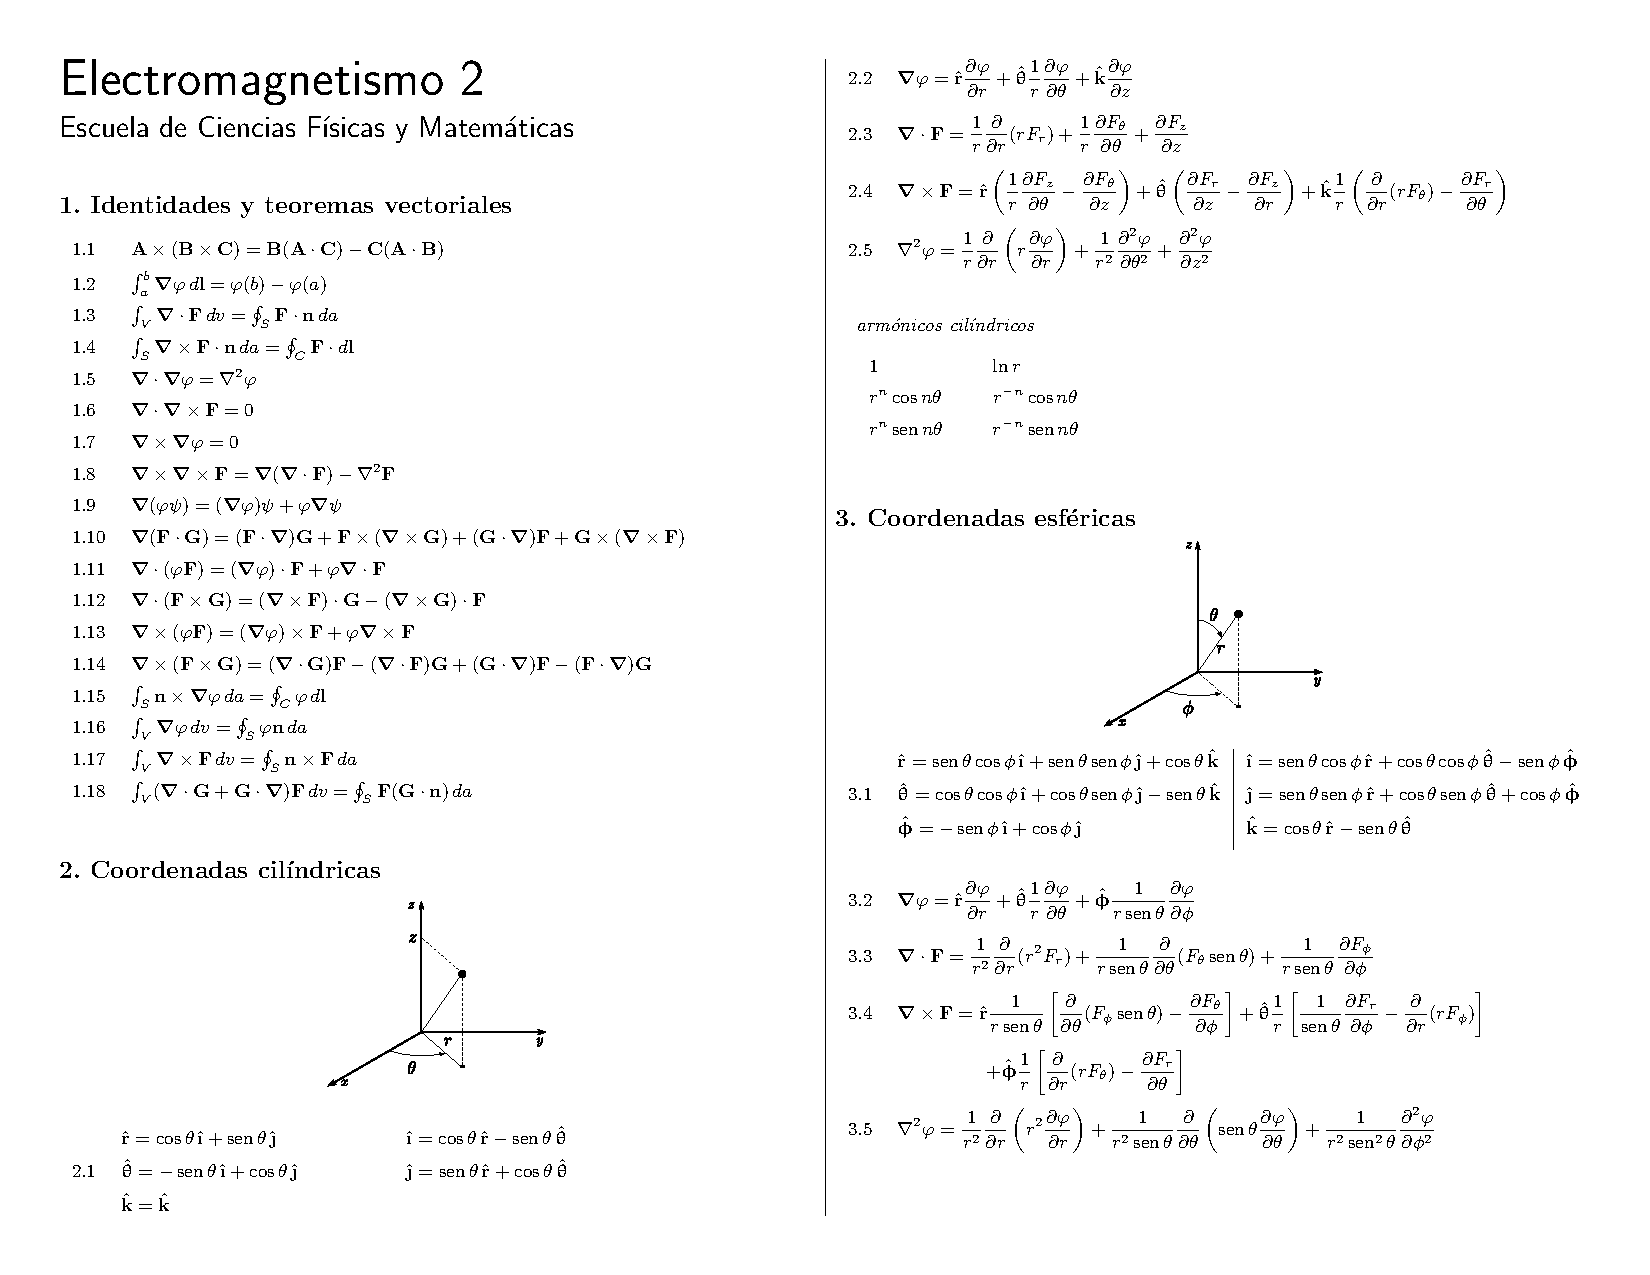
\includepdf[pages=-, scale=0.9]{./img/formulario_electro2.pdf}






































%%%%%%%%%%%%%%%%%